\chapter{实分析}
\section{基础微积分}
\begin{ans}
  令$f(\theta)=\cos(p\theta)-(\cos\theta)^p$. 我们有$f(0)=0$,且对$0<\theta<\pi/2$,
  \begin{align*}
    f'(\theta) & = -p\sin(p\theta) + p\cos^{p-1}\theta\sin\theta\\
    & = p\Big( -\sin(p\theta) +\frac{\sin\theta}{\cos^{1-p}\theta} \Big)\\
    & >0
  \end{align*}
  由于$\sin x$在$[0,\pi/2]$上单调递增,且$\cos^{1-p}\theta\in(0,1)$. 我们得到$0\le\theta\le\pi/2$时, $f(\theta)\ge0$,这就证明题中的不等式.
\end{ans}

\begin{ans}
  设$x\in[0,1]$. 根据$f(0)=0$,利用Cauchy-Schwarz不等式,我们有
  \begin{align*}
    |f(x)| & = \Big|\int_0^x f'(t)\,\mathrm dt \Big|\\
           & \le \sqrt{\int_0^x|f'(t)|^2\,\mathrm dt}
           \sqrt{\int_0^x1^2\,\mathrm dt}\\
           & \le \sqrt{\int_0^x|f'(t)|^2\,\mathrm dt},
  \end{align*}
  结论得证.
\end{ans}

\begin{ans}
  由于$f'$为正, $f$是增函数,所以对$t>1$,我们有$f(t)>f(1)=1$. 因此,对$t>1$,
  \[ f'(t) =\frac1{t^2+f^2(t)}<\frac1{t^2+1}, \]
  因此
  \begin{align*}
    f(x) & = 1 + \int_1^xf'(t)\,\mathrm dt\\
         & < 1 + \int_1^x\frac1{t^2+1}\,\mathrm dt\\
         & < 1 + \int_1^{+\infty}\frac1{t^2+1}\,\mathrm dt\\
         & = 1+ \frac\pi4.
  \end{align*}
  所以$\lim_{x\to+\infty}f(x)$存在,且不会超过$1+\pi/4$. 严格的不等号成立,是因为
  \begin{align*}
    \lim_{x\to+\infty}f(x) & = 1 + \int_1^{+\infty}f'(t)\,\mathrm dt\\
     & < 1 + \int_1^{+\infty}\frac1{t^2+1}\,\mathrm dt
     = 1 + \pi/4.
  \end{align*}
\end{ans}

\begin{ans}
  用$M$表示$f$和$g$的共同上界. 由于$f$和$g$都是连续的,而$[0,1]$为紧集,因此存在$\alpha,\beta\in[0,1]$,使得$f(\alpha)=g(\beta)=M$. 定义函数$h(x)=f(x)-g(x)$,则它满足$h(\alpha)=M-g(\alpha)\ge0,h(\beta)=f(\beta)-M\le0$. 由于$h$是连续的,它必然在$\alpha$与$\beta$之间存在零点$t\in[0,1]$. 那么我们有$f(t)=g(t)$,所以$f^2(t)+3f(t)=g^2(t)+3g(t)$.
\end{ans}

\begin{ans}
  称具有题中形式的函数为一个{\kaishu 周期多项式},如果其中$x^k$是具有非零系数的次数最大的项,则称其{\kaishu 度}为$k$.

  如果$a$是1- 周期的,则$\Delta(af)=a\Delta f$对任意$f$成立,所以,由归纳法可知,$\Delta^n(af)=a\Delta^nf,\forall n$.

  我们将用完全归纳法证明结论. 对$n=1$,结论成立:$\Delta f=0$当且仅当$f$是1- 周期的. 假定结论对$1,\cdots,n-1$已经成立,如果
  \[ f = a_0+a_1x+\cdots+a_{n-1}x^{n-1} \]
  是一个度至多为$n-1$的周期多项式,则
  \[ \Delta f = a_1\Delta^nx+\cdots+a_{n-1}\Delta^n (x^{n-1}). \]
  而归纳假设说明,所有项中除了可能的最后一项之外,其他项全部为零. 我们有$\Delta^n(x^{n-1})=\Delta^{n-1}\Delta(x^{n-1})$,由二项式定理知这是一个度为$n-2$的多项式. 所以归纳假设也意味着$\Delta^n(x^{n-1})=0$,于是充分性得证.

  对于必要性,假定$\Delta^nf=0$. 由归纳假设,$\Delta f$是一个度不超过$n-2$的周期多项式. 假定我们能找到一个周期多项式$g$,其度不超过$n-1$,使得$\Delta g=\Delta f$. 则由$\Delta(f-g)=0$,可知函数$f-g$是1- 周期的,这意味着$f$是一个周期多项式,且其度不超过$n-1$,正好满足题意. 因此,只需要证明如下断言: 如果$h$是一个度为$n(n=0,1,\cdots,n)$的周期多项式,那么存在一个度为$n+1$的周期多项式,使得$\Delta g=h$.

  如果$n=0$,我们取$g=hx$. 假定$h$的度$n>0$,且假定断言对度小于$n$的情形已经成立. 那么不失一般性,我们可以假定$h=ax^n$,这里$a$是1- 周期的. 由二项式定理,
  \[ h-\Delta\bigg( \frac{ax^{n+1}}{n+1} \bigg) \]
  是一个度为$n-1$的周期多项式,那么它等于$\Delta g_1$,而$g_1$是某个度为$n$的周期多项式,并且我们有$h=\Delta g$,这里
  \[ g=\frac{ax^{n+1}}{n+1}+g_1, \]
  得证.
\end{ans}

\begin{ans}
  由于$f$是递增的,且非常值,那么存在$r_0<s_0$使得$f(r_0)<f(s_0)$. 我们不妨假定$\delta=s_0-r_0>1$. 令$\Delta=f(s_0)-f(r_0)$.

  取$[r_1,s_1]$或者是$[r_0,(r_0+s_0)/2]$,或者是$[(r_0+s_0)/2,s_0]$,使得$f(s_1)-f(r_1)$较大(如果他们相等则任取一个即可). 则$f(s_1)-f(r_1)\ge\Delta/2$. 类似地取$[r_2,s_2]$是$[r_1,s_1]$的左半或右半区间,使得$f(s_2)-f(r_2)$较大. 不停地取下去,则$s_i-r_i=2^{-i}\delta$,且$f(s_i)-f(r_i)\ge2^{-i}\Delta$.

  令$a=\lim r_i$,且设$c=\Delta/(2\delta)$. 给定$x\in(0,1]$,取第一个使得$2^{-i}\delta\le x$的整数$i\ge0$. 则$2^{-i}\delta\ge x/2$. 区间$[r_i,s_i]$包含点$a$,且其长度$\le x$,所以$[r_i,s_i]\subset[a-x,a+x]$. 由于$f$递增,
  \[ f(a+x)-f(a-x)\ge f(s_i)-f(r_i)\ge2^{-i}\Delta=2c2^{-i}\delta\ge cx. \]
  最后,不等式$f(a+x)-f(a-x)\ge cx$对$x=0$显然成立.
\end{ans}

\begin{ans}
  \begin{enumb}
    \item 错误. 对于
  \end{enumb}
  \[ f(t)=g(t)=\begin{cases}
    0, &t\ne0\\
    1, &t=0
  \end{cases}, \]
  我们有$\lim_{t\to0}g(t)=\lim_{t\to0}f(t)=0$,但
  $\lim_{t\to0}f\big(g(t)\big)=1$.\\
  \begin{enumb}\setcounter{enumi}{1}
    \item 错误. $f(t)=t^2$将开区间$(-1,1)$映为$[0,1)$,这不是开的.
    \item 正确. 设$x,x_0\in(-1,1)$. 由Taylor定理,存在$\xi\in(-1,1)$使得
  \end{enumb}
        \[
          f(x) = \sum_{k=0}^{n-1}\frac{f^{(k)}(x_0)}{k!}(x-x_0)^k
          +\frac{f^{(n)}(\xi)}{n!}(x-x_0)^n\quad(n\in\MN).
        \]
      我们有
      \[ \lim_{n\to\infty}\bigg| \frac{f^{(n)}(\xi)}{n!}(x-x_0)^n \bigg| \le
      \lim_{n\to\infty}\frac{|x-x_0|^n}{n!}=0,\]
      所以
      \[ f(x) = \sum_{k=0}^{\infty}\frac{f^{(k)}(x_0)}{k!}(x-x_0)^k
      \]
      对任意$x_0\in(-1,1)$都成立,即$f$是实解析的.
\end{ans}

\begin{ans}
  \method 令$f(x)=\sin x-x-x^3/6$,则$f(0)=f'(0)=f''(0)=0$,且$f'''(x)=1-\cos x$,于是$f'''(x)\ge0,\forall x$,且对$0<x<2\pi$,有$f'''(x)>0$. 于是对$x>0$,有$f''(x)=\int_0^xf'''(t)\,\mathrm dt>0$. 类似地, $f'(x)=\int_0^xf''(t)\,\mathrm dt>0$,那么最后$f(x)=\int_0^xf'(t)\,\mathrm dt>0$.

  \method 令$f(x)=\sin x-x-x^3/6$,则
  \begin{align*}
    f'(x) & = \cos x -1 +\frac{x^2}2,\\
    f''(x) & = -\sin x + x,\\
    f'''(x) & = -\cos x + 1.
  \end{align*}
  现在$f'''(x)\ge0$,且等号只在离散的点$2n\pi,n\in\MZ$处取到, 因此$f''$在$\MR$上严格递增. 由于$f''(0)=0$,我们得到$f''(x)>0,\forall x>0$,因此$f'$在$\MR^+$上严格递增. 由于$f'(0)=0$,我们得到$f'(x)>0,\forall x>0$,因此$f$在$\MR^+$上严格递增. 由于$f(0)=0$,我们得到$f(x)>0,\forall x>0$,证毕.

  \method 考虑$\sin x$在$0$处的带Lagrange余项的5阶Taylor展开,对$x>0$,我们有
  \[
    \sin x = x-\frac{x^3}+\frac{x^5}{5!}+\frac{\cos^6\xi}{6!},
  \]
  这里$\xi\in(0,x)$. 由于$x^5/5!>0$,且$\cos^6\xi/6!\ge0$,那么原不等式成立.
\end{ans}

\begin{ans}
  $\sin x$的3阶Maclaurin展开式为
  \[ \sin x=x-\frac{x^3}6+O(x^5),\quad x\to0, \]
  因此
  \[ \sin^2x = x^2+O(x^4),\quad x\to0. \]
  因此,当$h$在$0$的邻域范围内时,我们有$y(h)=1-8\pi^2h^2+O(h^4)$ (或者,注意到$y(h)=\cos(4\pi h)$,然后利用余弦函数的展开式). 因此
  \begin{align*}
    f\big(y(h)\big) & = \frac2{1+\sqrt{8\pi^2h^2+O(h^4)}} \\
       & = \frac2{1+2\sqrt2\pi|h|+O(h^2)},\quad h\to0.
  \end{align*}
  利用Maclaurin展开式$2/(1+x)=2-2x+2x^2+O(x^2)$,我们得到
  \[ f\big(y(h)\big)=2-4\sqrt2\pi|h|+O(h^2),\quad h\to0. \]
\end{ans}

\begin{ans}
  \begin{enumb}
    \item 设$f:[0,1]\to(0,1)$是一个连续的满射. 考虑序列$(x_n):x_n\in f^{-1}\big((0,1/n)\big)$. 由Balzono-Weierstrass定理,我们可以假定$(x_n)$收敛到某个$x\in[0,1]$. 由连续性,我们有$f(x)=0$,这是不可能的. 因此,这样的函数不存在.
    \item 取$g(x)=|\sin2\pi x|$即可.
    \item 设$g:(0,1)\to[0,1]$是一个连续的双射,令$x_0=g^{-1}(0),x_1=g^{-1}(1)$. 不失一般性,假定$x_0<x_1$(否则考虑$1-g$). 由介值定理,我们有$g([x_0,x_1])=[0,1]$. 而$x_0,x_1\in(0,1)$,那么$g$不是单射,矛盾.
  \end{enumb}
\end{ans}

\begin{ans}
  令$A(c)$表示题中所指区域的面积. $f''>0$意味着$f$是凸函数,因此$f$的图像总是在其切线的上方,且我们有
  \[ A(c)=\int_a^b\big( f(x)-f(c)-f'(c)(x-c)\big)\,\dx. \]
  $A$的导数为
  \begin{align*}
    A'(c) & = - \int_a^b f''(c)(x-c)\,\dx\\
          & = -f''(c)\frac{b^2-a^2}2 +(b-a)cf'(c)\\
          & = f''(c)(b-a)\Big( c-\frac{a+b}2 \Big),
  \end{align*}
  因此极小值在$c=(a+b)/2$处取到. 而$A'$是单调递增的, $A$是凸函数,因此$A$在$[a,b]$上的最小值只在$c=(a+b)/2$处取到.
\end{ans}

\begin{ans}
  \method 利用椭圆的参数方程
   \[ x=a\cos t,\quad y=b\sin t, \]
  椭圆上的三个点可以表示为
   \[ (a\cos t_i,b\sin t_i),\quad i=1,2,3. \]
  因此,内接三角形的面积可表示为
   \[
     \frac12\begin{vmatrix}
       1 & a\cos t_1 & b\sin t_1\\
       1 & a\cos t_2 & b\sin t_2\\
       1 & a\cos t_3 & b\sin t_3
     \end{vmatrix} = \frac{ab}2
     \begin{vmatrix}
       1 & \cos t_1 & \sin t_1\\
       1 & \cos t_2 & \sin t_2\\
       1 & \cos t_3 & \sin t_3
     \end{vmatrix},
   \]
  它等于单位圆内接三角形面积的$ab$倍. 在圆的情形下,给定在所有的内接三角形中,如果给定底边长为$2w(0<w\le1)$,其面积在等腰三角形的情形时最大,此时面积为
  \[ g(w) = w\big( 1+\sqrt{1-w^2} \big). \]
  容易知道$g$在区间$[0,1]$上的最大值在$w=\sqrt3/2$处取到,此时恰为一个等边三角形,且面积为$3\sqrt3/4$. 或者,固定三角形的一边为底,我们很容易知道,在所有的内接三角形中,具有最大面积的三角形是等腰三角形,因为此时的高是最大的,说明底边上的两个角是一样的. 固定另一条边为底,我们发现此三角形也当然是等腰的. 因此,面积的最大值在
  \[ t_2=t_1+\frac{2\pi}3\quad \text{和} \quad t_3=t_2+\frac{2\pi}3 \]
  时取到. 这时,相应的内接于单位圆的三角形是等边的.

  对于半轴长分别为$a,b$的椭圆,相应的内接三角形面积的最大值为$3ab\sqrt3/4$.

  \method 设$f:\MR^2\to\MR^2$为伸缩函数$f(x,y)=(ax,by)$. 根据积分的换元公式,我们有
  \[ \vol\big(f(T)\big) = |\det f|\cdot\vol(T). \]
  由于$f$的行列式为常数,接着之前证明的步骤,最大面积在等边三角形时取到,且其面积为
  \[ \vol\big(f(T)\big) = ab\cdot\vol(T)=3ab\frac{\sqrt3}4. \]
\end{ans}

\begin{ans}
  假定$a,b$都在$A$中,且$a<b$, 设$a<c<b$. 令$(x_n)$和$(y_n)$是$[0,+\infty)$中的两个趋于$+\infty$数列,分别满足$a=\lim_{n\to+\infty}f(x_n)$和$b=\lim_{n\to+\infty}f(y_n)$. 如果有必要的话,从两个数列中各删除有限项,我们可以假定$f(x_n)<c$且$f(y_n)>c,\forall n$. 那么由介值定理,对每个$n$都存在介于$x_n$和$y_n$之间的点$z_n$,使得$f(z_n)=c$. 且显然$\lim_{n\to+\infty}z_n=+\infty$,因此$c\in A$,证毕.
\end{ans}

\begin{ans}
  对每个$x>0$,从方程$x\big( 1+\ln (1/\varepsilon\sqrt x) \big)=1$中解出$\varepsilon$得$\varepsilon=\ee/(x^{1/2}\ee^{1/x})$,我们将右边设为$f(x)$.

  对$x>0$,定义$g(x)=x^{1/2}\ee^{1/x}=\ee/f(x)$, 则$g'(x)=x^{-3/2}\ee^{1/x}(x-2)/2$. 于是$g$在$(0,2]$上严格递减,且$[2,+\infty)$上严格递减. 进一步,有$\lim_{x\to0^+}g(x)=+\infty=\lim_{x\to+\infty}g(x)$,且$g(2)>0$,因此$\lim_{x\to0^+}f(x)=0=\lim_{x\to+\infty}f(x)$, $f$在$(0,2]$上严格递增,在$[2,+\infty)$上严格递减,在$(0,+\infty)$上连续,且$f(2)=\sqrt{\ee/2}$. 分别用$f_1,f_2$表示$f$在$(0,2)$和$(2,+\infty)$上的限制. 则对每个$0<\varepsilon<\sqrt{\ee/2}$,给定的方程恰有两个解,即$x=f_1^{-1}(\varepsilon),x_2=f_2^{-1}(\varepsilon)$, 较小的解即为$x=f_1^{-1}(\varepsilon)$. 由于$f_1$是严格单调递增且连续的,且$f(0^+)=0$,我们推出$\varepsilon\to0^+$时, $x(\varepsilon)\to0$.

  固定$s>0$,现在$\varepsilon^{-s}x(\varepsilon)
  =(\ee/x^{1/2}\ee^{1/x})^{-s}x=\ee^{-s}x^{1+s/2}x\ee^{s/x}$,这里$x=x(\varepsilon)=f_1^{-1}(\varepsilon)$. 当$\varepsilon\to0^+$时,$x\to0^+$. 而函数$x\mapsto
  \ee^{-s}x^{1+s/2}\ee^{s/x}$在$x\to0^+$时的极限为$+\infty$,这就证明了第二部分.
\end{ans}

\begin{ans}
  设$g$是一个多项式,
  \[ g(x)=a_0+a_1(x-a)+a_2(x-a)^2+\cdots+a_n(x-a)^n. \]
  如果我们取
  \[ a_0=\frac1{f(a)},\quad a_1=-\frac{f'(a)g(a)}{f(a)},
  \quad a_2=-\frac{f''(a)g(a)+f'(a)g'(a)}{f(a)}, \]
  直接计算可以验证$g$满足题意.
\end{ans}

\begin{ans}
  假定$p$的所有根都是实根,令$\deg p=n$. 我们有
  \[ p(z)=(z-r_1)^{n_1}(z-r_2)^{n_2}\cdot(z-r_k)^{n_k}, \]
  这里$r_1<r_2<\cdots<r_k$,且$\sum_{i=1}^k n_i=n$. 对上式求导,我们可知当$n_i>1$时, $r_i$是$p'$的$n_i-1$重根. 将这些重数相加,我们发现已经找到了$p'$的$n-1$个根中的$n-k$个. 现在由Rolle定理,对每个$i,1\le i\le k-1$,存在点$s_i,r_i<s_i<r_{i+1}$,使得$p'(s_i)=0$. 因此,我们找到了$p'$剩下的$k-1$个根,并且它们是互异的. 现在我们知道$a$是$p'$的根而不是$p$的根,因此$a\ne r_i,\forall i$. 但$a$时$p''$的根,所以$a$一定是$p'$的重根,因此$a\ne s_i,\forall i$. 所以,$a$不是$p'$的根,矛盾.
\end{ans}

\begin{ans}
  设$x\in\MR$且$h>0$. 由Taylor定理,存在$w\in(x,x+2h)$使得
  \[ f(x+2h)=f(x)+2hf'(x)+2h^2f''(w), \]
  或者写为
  \[ f'(x)=\frac{f(x+2h)-f(x)}{2h} -hf''(w). \]
  取绝对值,然后利用题设条件,我们有
  \[|f'(x)|\le \frac Ah+hB.\]
  现在令$h=\sqrt{A/B}$,即得到
  \[ |f'(x)|\le2\sqrt{AB}. \]
\end{ans}

\begin{ans}
  \method 考虑函数$f(x)=\ln x/x$, 我们有$a^b=b^a$当且仅当$f(a)=f(b)$. 现在$f'(x)=(1-\ln x)/x^2$,所以$f$对$x<\ee$递增,对$x>\ee$递增. 要想题中的等式成立,一定有$0<a<\ee$,因此$a$是$1$或$2$,且$b>\ee$. 对$a=1$,显然是无解的. 对$a=2$, 则$b=4$满足. 而$f$在$x>\ee$时递减,因此这就是唯一的解.

  \method 显然, $a,b$具有相同的素因子. 令$b=a+t$,这里$t$是某个整数. 于是$a^aa^t=b^a$,这意味着$a^a|b^a$,于是$a|b$,那么$b=ka$, $k$是某个大于1的整数. 现在$b^a=(ka)^a=a^b$,则意味着$k$是$a$的某个幂次,因此$b=a^m$,$m$是某个大于1的整数. 现在$b^a=a^{ma}=a^{a^m}$,当且仅当$ma=a^m$,显然可知此时只有唯一解$a=m=2$,因此$a=2,b=2^2=4$.

  \method 令$b=a(1+t)$,$t$是某个正数. 则方程$a^b=b^a$等价于以下任意一个式子:
  \begin{gather*}
    a^{a(1+t)} = \big(a(1+t)\big)^a,\\
    (a^a)^{1+t} = a^a(1+t)^a,\\
    (a^a)^t = (1+t)^a,\\
    a^t = 1+t.
  \end{gather*}
  由指数函数的幂级数展开可知$\ee^t>1+t$对$t>0$成立,也就是对$a<\ee$成立. 而$a=1$是不可能,必有$a=2$. 最初的方程则变为
  \[ 2^b=b^2, \]
  考虑$b$的素因子分解,显然可得$b=4$.
\end{ans}

\begin{ans}
  原方程可写为$a^{x^b}=x$,或者
  \[ \frac{\ln x}{x^b} = \ln a. \]
  此方程有解,当且仅当$\ln a$在函数$x\mapsto (\ln x)/x^b$的值域内. 不难得知此函数的值域是$(-\infty,1/b\ee]$. 因此,原方程有解,当且仅当$1<a<\ee^{1/b\ee}$.
\end{ans}

\begin{ans}
  \method 令$f(x)=3^xx^{-3},x>0$,我们有
  \[ f'(x)=\frac{3^x(x\ln3-3)}{x^4}>0,\quad x>\frac{3}{\log3}. \]
  由于$3/\log3<3<\pi$,我们有$f(3)=1<f(\pi)=3^\pi/\pi^3$,即$\pi^3<3^\pi$.

  \method 可以对函数$f(x)=\ln(x)/x$进行同样的分析,此函数对$x>\ee$递减. 也可以考虑函数$g(x)=x^3-3^x$和$h(x)=(3+x)^{\pi-x}$.
\end{ans}

\begin{ans}
  固定$a\in(1,+\infty)$,在$(1,+\infty)$上考虑函数$f(x)=a^xx^{-a}$,我们尝试求出其最小值. 由于$\ln f(x)=x\ln a-a\ln x$,我们
  \[ \frac{f'(x)}{f(x)} = \ln a - \frac ax, \]
  说明$f'(x)$在$(1,a/\ln a)$上为负,在$(a/\ln a,+\infty)$上为正. 因此,$f$在$(1,+\infty)$上的最小值在$x_a=a/\ln a$处取到,且
  \[ \ln f(x_a)=a-a\ln\Big(\frac a{\ln a} \Big)
  = a \ln\Big( \frac{\ee\ln a}a \Big).\]
  要想$a$满足题中的条件,当且仅当$\ee\ln a/a\ge1$. 要得到哪个$a$满足条件,在$(1,+\infty)$上考虑函数$g(y)=\ln y/y$,我们有
  \[ g'(y)=\frac{1-\ln y}{y^2}, \]
  由此可知$g$在$(1,+\infty)$上的最大值在$y=\ee$处取到,最大值为$g(\ee)=1/\ee$. 由于在$(1,+\infty)\backslash\ee$上,$g(y)<1/\ee$,我们得知$\ee\ln a/a<1$对任意$a\in(1,+\infty)\backslash\ee$成立,因此$a=\ee$是$(1,+\infty)$上唯一的满足条件的数.
\end{ans}

\begin{ans}
  令$g(x)=\ee^x/x^t,x>0$. 由于当$x\to0$和$x\to+\infty$时,均有$g(x)\to+\infty$,因此在中间必有一个最小值. 在最小值处,
  \[ g'(x)=\ee^xx^{-t}(1-t/x)=0, \]
  因此最小值在$x=t$处取到,此时
  \[ g(x)=g(t)=\ee^t/t^t=(\ee/t)^t. \]
  于是
  \[ \ee^x \ge \Big(\frac{x\ee}t \Big)^t, \]
  且右边的式子当且仅当$t<\ee$时,它严格大于$x^t$.
\end{ans}

\begin{ans}
  在区间$[-1,1]$上,$f$可以写成二阶Lagrange余项的Maclaurin多项式:
  \[
    f(x)=f(0)+f'(0)x+\frac{f''(0)}2x^2+\frac{f^{(3)}(\xi)}6x^3,
  \]
  其中$\xi$介于$0$与$x$之间. 在上式中令$x=\pm1/n$,并结合要证明的结果,我们有
  \begin{align*}
    n\bigg( f\Big(\frac1n\Big)-f\Big(-\frac1n\bigg) \Big)      -2f'(0)  & = n\bigg( \frac{2f'(0)}n+\frac{f^{(3)}(\alpha_n)}{6n^3}
    +\frac{f^{(3)}(\beta_n)}{6n^3}-2f'(0) \bigg)\\
    & = \frac{f^{(3)}(\alpha_n)+f^{(3)}(\beta_n)}{6n^2},
  \end{align*}
  这里$\alpha_n,\beta_n\in[-1,1]$. 由于$f'''$连续,存在$M>0$,使得$|f'''(x)|<M$对任意$x\in[-1,1]$成立,因此
  \[
    \sum_{n=1}^\infty\bigg|
    n\bigg( f\Big(\frac1n\Big)-f\Big(-\frac1n\Big) \bigg)      -2f'(0) \bigg|
    \le \frac M3\sum_{n=1}^\infty \frac1{n^2} <+\infty.
  \]
\end{ans}

\begin{ans}
  由Taylor定理,
  \[ f(x+h)-f(x)=f'(x)+\frac{f''(z)}2h^2, \]
  其中$z$介于$x$与$x+h$之间. 类似地,
  \[ f(x-h)-f(x)=-f'(x)h+\frac{f''(w)}2h^2, \]
  $w$介于$x$与$x-h$之间. 将两式相加,除以$h^2$,再令$h\to0$即证得所求结果.
\end{ans}

\begin{ans}
  \begin{enumb}
  \item 几何图形
  \end{enumb}
  \begin{figure}[ht]
    \centering
    \begin{tikzpicture}[>=Stealth,scale=2.5]
      \draw[->](-0.2,0) -- (0,0) node[below left]{$O$}
      -- (2,0) node[below]{$x$};
      \draw[->](0,-0.2) -- (0,1.3) node[right]{$y$};
      \fill(pi/2,0) circle(0.3pt) node[below]{$\pi/2$};
      \fill(0,1) circle(0.3pt) node[left]{$1$}
        (0,0) circle(0.3pt) (pi/2,1) circle(0.3pt);
      \draw[semithick](0,0) -- (pi/2,1);
      \draw[semithick,samples=200]plot[domain=0:1.7]
      (\x,{sin(\x r)});
      \node[rotate=36]at(0.7,0.77) {$y=\sin x$};
    \end{tikzpicture}
    \caption{\label{fig\theans}}
  \end{figure}

  \noindent 说明了
  \[ \sin\theta\ge\frac2\pi\theta,\quad 0\le\theta\le\frac\pi2. \]
  严格的分析证明可以通过$\sin\theta$在区间$[0,\pi/2]$上是凹函数(二阶导数为负)的事实来写.

  也可以通过下面的几何构造来说明(首先由 J\'ozsef S\'andor发现,后来由冯跃峰重新发现):
  \begin{figure}[!ht]
    \centering
    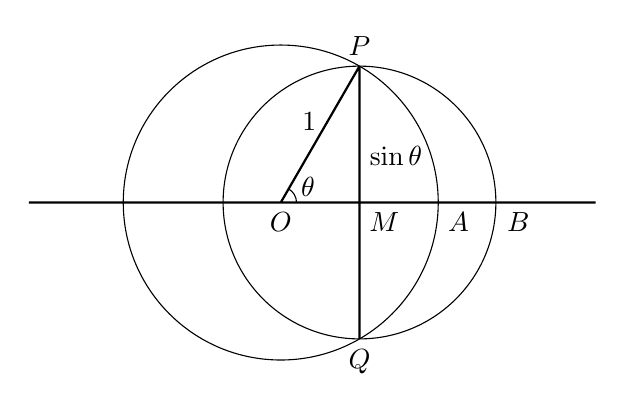
\begin{tikzpicture}[scale=2,rounded corners=0.4pt]
      \draw[thick] (-1.6,0) -- (2,0)
        (0,0)--node[above left,inner sep=1pt]{$1$}
        (0.5,{sqrt(3)/2})node[above]{$P$}
        --node[pos=0.33,right]{$\sin\theta$}
        (0.5,{-sqrt(3)/2})node[below]{$Q$};
      \draw(0,0)node[below]{$O$} circle(1);
      \draw(0.5,0)node[below right]{$M$}
      circle({sqrt(3)/2});
      \draw(1,0)node[below right]{$A$}
       (1.375,0)node[below right]{$B$};
      \draw(0.1,0) arc(0:60:0.1);
      \node at (30:0.2){$\theta$};
    \end{tikzpicture}
    \caption{\label{geo}}
  \end{figure}
  \begin{align*}
    OB = OM + MB \ge OM
    & \Rightarrow \wideparen{PBQ} \ge \wideparen{PAQ}\\
    & \Rightarrow \pi\sin\theta \ge 2\theta\\
    & \Rightarrow \sin\theta \ge \frac{2\theta}\pi.
  \end{align*}
  \begin{enumb}\setcounter{enumi}{1}
    \item \method 不等式
  \end{enumb}
    \begin{align*}
      J & = \int_0^{\frac\pi2}\ee^{-R\sin\theta}R\,\mathrm d\theta\\
        & \le \int_0^{\frac\pi2}\ee^{-2R\theta/\pi}R\,\mathrm d\theta\\
        & = -\pi\ee^{-2R\theta/\pi}\Big|_0^{\pi/2}\\
        & <\pi
    \end{align*}
    称为Jordan引理. 于是所求的极限为
    \begin{align*}
      \lim_{R\to+\infty}R^\lambda\int_0^{\frac\pi2}
      \ee^{-R\sin\theta}\,\mathrm d\theta
      & = \lim_{R\to+\infty}\int_0^{\frac\pi2}
      \ee^{-R\sin\theta}R\,\mathrm d\theta\\
      & <\lim_{R\to+\infty}R^{\lambda-1}\pi = 0.
    \end{align*}
    \method 我们有
    \[
      R^\lambda\int_0^{\frac\pi2}
      \ee^{-R\sin\theta}\,\mathrm d\theta =
      R^\lambda\int_0^{\frac\pi3}
      \ee^{-R\sin\theta}\,\mathrm d\theta +
      R^\lambda\int_{\frac\pi3}^{\frac\pi2}
      \ee^{-R\sin\theta}\,\mathrm d\theta.
    \]
    由于$0\le\theta\le\pi/3$时,$\cos\theta\ge1/2$,而$\sin\theta$在$[0,\pi/2]$上是增函数,我们有
    \begin{align*}
      R^\lambda\int_0^{\frac\pi2}
      \ee^{-R\sin\theta}\,\mathrm d\theta
      & \le 2R^\lambda\int_0^{\frac\pi3}
      \ee^{-R\sin\theta}\cos\theta\,\mathrm d\theta
      + R^\lambda\int_{\frac\pi3}^{\frac\pi2}
      \ee^{-R\sin(\pi/3)}\,\mathrm d\theta\\
      & = 2R^{\lambda-1}\Big( 1-\ee^{-R\sin(\pi/3)} \Big)
      + \frac{R^\lambda\pi}6\ee^{-R\sin(\pi/3)}\\
      & = o(1)\quad (R\to\infty).
    \end{align*}
\end{ans}

\begin{ans}
  设$T=\MR\backslash S$,由于每个非空区间都包含无穷个数,$T$在$\MR$中是稠密的.

  固定$p\in T$,定义$F:\MR\to\MR$,
  \[ F(x) = \int_p^xf(t)\,\mathrm dt. \]
  则$F$在$T$上恒为零,那么由$F$的连续性可知$F$在$\MR$上恒为零. 因此,我们就证明了$F'=f\equiv=0$.
\end{ans}

\begin{ans}
  由Rolle定理知,存在$c\in(0,1)$,使得$f'(c)=0$. 而$f$的凹性说明$f$在$(0,c)$上递增,在$(c,1)$上递减. $f$的图像在$[0,c]$上的弧长为
  \[
    L_{(0,c)} = \int_0^c\sqrt{1+[f'(x)]^2}\,\mathrm dx
    =\lim_{n\to\infty}\frac cn\sum_{k=0}^{n-1}
    \sqrt{1+[f'(\xi_k)]^2},
  \]
  其中$\xi_k\in \big(kc/n,(k+1)c/n\big)$. 由Lagrange中值定理,我们可以假定$\xi_k$满足
  \[ f'(\xi_k)=\frac{f\big((k+1)c/n\big)-f(kc/n)}{c/n}. \]
  由于$f$是递增的,我们得到
  \begin{align*}
    L_{(0,c)} & = \lim_{n\to\infty}\sqrt{
    (c/n)^2+\big[f\big( (k+1)c/n \big)-f(kc/n) \big]^2
    }\\
    & \le \lim_{n\to\infty}\sum_{k=0}^{n-1}
    \big[ c/n + f\big( (k+1)c/n \big)-f(kc/n) \big]\\
    & c + f(c).
  \end{align*}
  类似地,可得$L_{(c,1)}\le 1-c+f(c)$,所以$L_{[0,1]}\le c+f(c)
  +1-c+f(c)\le3$.
\end{ans}

\begin{ans}
  $\int_1^{+\infty}|f'(x)|\,\dx$收敛意味着$\int_1^{+\infty}f'(x)\,\dx$收敛,这说明极限$\lim_{x\to+\infty}f(x)$存在. 如果此极限不是0,那么$\sum_{n=1}^\infty f(n)$与$\int_1^{+\infty}f(x)\,\dx$均发散,因此我们可以假定$\lim_{x\to+\infty}f(x)=0$. 那么当$r\to+\infty$时, $\int_{\lfloor r\rfloor}^rf(x)\,\dx\to0$(这里$\lfloor r\rfloor$表示不超过$r$的最大整数),这意味着$\int_1^{+\infty}f(x)\,\dx$收敛当且仅当极限$\lim_{n\to\infty}f(x)\,\dx$(这是$n$是正整数)存在. 换句话说, $\int_1^{+\infty}f(x)\,\dx$的收敛性等价于$\sum_{n=1}^\infty \int_n^{n+1}f(x)\,\dx$的收敛. 因此,只需要证明
  \[ \sum_{n=1}^\infty\Big|\int_n^{n+1}f(x)\,\dx -f(n) \Big|
  <+\infty. \]
  我们有
  \begin{align*}
    \bigg|\int_n^{n+1}f(x)\,\dx -f(n) \bigg|
    & = \bigg| \int_n^{n+1}\big( f(x)-f(n) \big) \bigg| \\
    & = \bigg| \int_n^{n+1}\int_n^xf'(t)\,\mathrm dt\,\dx \bigg|\\
    & \le \int_n^{n+1}\int_n^{n+1}|f'(t)|\,\mathrm dt\,\dx\\
    & = \int_n^{n+1}|f'(t)|\,\mathrm dt.
  \end{align*}
  因此
  \[ \sum_{n=1}^\infty\bigg|\int_n^{n+1}f(x)\,\dx -f(n) \bigg|
  < \int_1^{+\infty}|f'(t)|\,\mathrm dt <+\infty, \]
  得证.
\end{ans}

\begin{ans}
  我们有
  \[ |u(x)| = |u(x)-u(0)| \le |x|, \]
  且
  \[ |u^2(x)-u(x)| = |u(x)|\,|u(x)-1|\le |x|(|x|+1), \]
  所以
  \[ |\varphi(u)| \le \int_0^1|u^2(x)-u(x)|\,\dx
  \le \int_0^1x(x+1)\,\dx=\frac56. \]
  等号成立当且仅当$|u(x)|=x$且$|u(x)-1|=x+1$,也就是$u(x)=-x$,这刚好在$E$中.
\end{ans}

\begin{ans}
  由题意有
  \begin{align*}
    J(f) & =  \int_0^1f(x)\,\dx
    = \int_0^1\int_0^x f'(t)\,\mathrm dt \,\dx\\
    & = \int_0^1\int_t^1f'(t)\,\dx\,\mathrm dt
    = \int_0^1(1-t)f'(t)\,\mathrm dt.
  \end{align*}
  利用Cauchy-Schwarz不等式得
  \begin{align*}
    |J(f)|^2 & = \bigg(\int_0^1(1-t)f'(t)\,\mathrm dt\bigg)^2\\
    & \le \int_0^1(1-t)^2\,\mathrm dt\int_0^1[f'(t)]^2\,\mathrm dt \\
    & = \frac13\int_0^1[f'(t)]^2\,\mathrm dt\le \frac13,
  \end{align*}
  等号成立当且仅当$f'(t)=\sqrt3(1-t)$,此时$f(x)=\sqrt3(x-x^2/2)$. 即$J$在$S$上有上界,其上确界为$\sqrt3/3$,且在$f_0(x)=\sqrt3(x-x^2/2)$时取到其最大值.
\end{ans}

\begin{ans}
  令
  \[ u(t) = 1+2\int_0^tf(s)\,\mathrm ds. \]
  我们有
  \[ u'(t) = 2f(t) \le 2\sqrt{u(t)}, \]
  所以
  \[ \sqrt{u(t)}-1 = \int_0^t\frac{u'(s)}{2\sqrt{u(s)}}\,\mathrm ds
  \le \int_0^t\mathrm ds=t, \]
  因此
  \[ f(t)\le\sqrt{u(t)} \le 1+t. \]
\end{ans}

\begin{ans}
  我们将证明一定有$b=0$. 通过减去或者乘以常数,我们可以假定$a=0\le b$. 给定$\varepsilon>p$,取$R\ge1$使得对任意$x\ge R$,有
  \[ |\varphi(x)|\le\varepsilon \]
  且
  \[ \varphi'(x)\ge b/2\ge0. \]
  由微积分基本定理得
  \[ \varphi(x)=\varphi(R)+\int_R^x\varphi'(x)\,\dx, \]
  所以
  \[ 2\varepsilon\ge\varphi(x)-\varphi(R)
  \ge\int_R^x\frac b2\,\dx=(x-R)b/2. \]
  取$x=5R$,我们得到
  \[ b\le\varepsilon/R\le\varepsilon. \]
  由于$\varepsilon>0$是任意的,因此必有$b=0$.
\end{ans}

\begin{ans}
  设$0\le k_1<k_2<1$,则对任意$x\in(0,\pi/2)$,
  \begin{align*}
    -k_1\cos^2x & > - k_2\cos^2x,\\
    \sqrt{1-k_1\cos^2x} & > \sqrt{1-k_2\cos^2x},\\
    \frac1{\sqrt{1-k_1\cos^2x}} &< \frac1{\sqrt{1-k_2\cos^2x}},\\
    \int_0^{\frac\pi2}\frac1{\sqrt{1-k_1\cos^2x}}\,\dx
    & < \int_0^{\frac\pi2}\frac1{\sqrt{1-k_2\cos^2x}}\,\dx.
  \end{align*}
\end{ans}

\begin{ans}
  利用变量替换$y=x\sqrt t$,我们有
  \begin{align*}
    f(t) & = \int_{-\infty}^{+\infty} \ee^{-tx^2}\,\dx
    = \int_{-\infty}^{+\infty}\ee^{-y^2}\frac{\dy}{\sqrt t}\\
    & = \frac1{\sqrt t}\int_{-\infty}^{+\infty}\ee^{-y^2}\,\dy
    =\sqrt{\frac\pi t},
  \end{align*}
  所以
  \[ f'(t)=-\frac{\sqrt\pi}2t^{-3/2}. \]
\end{ans}

\begin{ans}
  令
  \[ G(u,v,x) = \int_v^u\ee^{t^2+xt}\,\mathrm dt, \]
  则$F(x)=G(\cos x,\sin x,x)$,所以
  \begin{align*}
    F'(x) & = \pp Gu\pp ux +\pp gv \pp vx+ \pp Gx\\
          & = \ee^{u^+xu}(-\sin x)-\ee^{v^+xv}\cos x
          +\int_v^ut\ee^{t^+xt}\,\mathrm dt,
  \end{align*}
  且
  \[ F'(0)=-1+\int_0^1t\ee^{t^2}\,\mathrm dt=\frac12(\ee-3). \]
\end{ans}

\begin{ans}
  \method \begin{enumb}
    \item 设$f(z)\ne0$,则
  \end{enumb}
  \[ f(x)f(z)=f\Big( \sqrt{x^2+z^2} \Big)
  =f(-x)f(z), \]
  所以$f(x)=f(-x)$,且$f$是偶函数. 而且$f(0)f(z)=f(z)$,所以$f(0)=1$.
  \begin{enumb}\setcounter{enumi}{1}
    \item 我们将用数学归纳法来证明$f(\sqrt nx)=f^n(x)$对$x\in\MR$和$n\in\MN$成立. 结论对$n=1$显然成立,假定结论对$n=k$ 成立,我们有
  \end{enumb}
        \begin{align*}
          f\Big(\sqrt{k+1}x\Big) & =
          f\bigg( \sqrt{\Big(\sqrt kx\Big)^2+x^2 }\bigg)\\
          & = f\Big(\sqrt kx\Big) f(x)=f^k(x)f(x)=f^{k+1}(x).
        \end{align*}
        如果$p,q\in\MN$,则
        \[ f(p)=f\Big(\sqrt{p^2}\cdot 1\Big)=[f(1)]^{p^2}, \]
        且
        \[ f(|p|) = f\Big( \sqrt{q^2}\cdot|p/q| \Big)
        =\big( f(|p/q|) \big)^{q^2}, \]
        由此得到
        \[ \big( f(p/q) \big)^{q^2}= \big(f(1)\big)^{p^2}. \]
        \begin{itemize}
          \item 如果$f(1)>0$,我们有
            \[ f(p/q)=\big(f(1)\big)^{p^2/q^2}, \]
            于是由$f$在$\MR$上的连续性可得
            \[ f(x)=\big(f(1)\big)^{x^2}. \]
          \item 如果$f(1)=0$,则$f$在$\MR$的 一个稠密集上恒为零,因此它在任意点均为零,与题设矛盾.
          \item 要说明$f(1)<0$不可能成立,只需考虑$q$为偶数而$q$为奇数,我们有$f(p/q)>0$,所以$f$在$\MR$的一个稠密集上恒为正,那么$f(1)\ge0$.
        \end{itemize}

    注意到我们只运用了$f$的连续性和它的函数方程.

    求导容易验证$f$满足所给的微分方程. 于是,满足条件的一般函数为
    \[ c^{x^2}, \]
    其中$0<c<1$.

  \method \begin{enumb}
    \item 取$x=y=0$,得$[f(0)]^2=f(0)$,因此$f(0)=0$或1. 如果$f(0)=0$,则对任意$x$有$0=f\big(\sqrt{x^2}\big)$,因此$f(x)=0,\forall x>0$. 如果存在$y$使得$f(y)\ne 0$,则$f(x)f(y)=0$意味着$f(x)=0,\forall x$. 因此只要$f(0)=0$,那么有$f(x)\equiv0$. 由于我们题设中$f$是非零的,因此必有$f(0)=1$. 在函数方程中取$y=0$,我们得到$f(x)=
        f\big(\sqrt{x^2}\big)=f(-x)$,所以$f$为偶函数.
    \item 等式两边关于$y$求导可得
    \end{enumb}
      \[ f(x)f'(y)=f'(r)r_y, \]
      这里$r=\sqrt{x^2+y^2}$,而$r_y$表示$r$对$y$的偏导数. 再次求导得
      \[ f(x)f''(y) = f''(r)r_y^2 + f'(r)r_{yy}. \]
      由于$r_y=y/r$且$r_{yy}=x^2/r^3$,取$y=0$我们得到
      \[ f'(x)=f''(0)xf(x), \]
      此微分方程的解为
      \[ f(x)=\ee^{f''(0)x^2/2}. \]
      由于$f$在无穷远处取零,必有$f''(0)/2=-\gamma<0$. 因此$f(x)=\ee^{-\gamma x^2}$,这里$\gamma$是某个正的常数.
\end{ans}

\begin{ans}
  设$C$是所有使得$\varepsilon_n=1$或$-1$的序列$\varepsilon=(\varepsilon_n)_1^\infty$构成的集合,它是一个不可数集. 对$\varepsilon\in C$,令$f_\varepsilon$表示$[0,1]$上的满足如下条件的函数:
  \begin{enumerate}
    \item $f_\varepsilon(0) = 0$;
    \item\label{1.1.37.2} 对任意正整数$n$,有$f_\varepsilon(1/n)=\varepsilon_n/n$;
    \item 在每个区间$[1/(n+1),1/n]$上,$f_\varepsilon$是一个线性函数,其端点值就是 \ref{1.1.37.2} 中所给的值.
  \end{enumerate}

  每个函数$f_\varepsilon$都是连续的: $f_\varepsilon$在$(0,1]$上的连续显然,而在$0$处连续性由$|f(x)|\le x$可得. 每个$f_\varepsilon$在有理点处取有理值,如果$x$是点$a=1/(n+1)$和$b=1/n$之间的一个有理点,则$x=(1-t)a+tb$,这里$t$是$[0,1]$上的某个有理数. 因此由$f_\varepsilon(a)$和$f_\varepsilon(b)$均为有理数可知$f_\varepsilon(x)=(1-t)f_\varepsilon(a)+tf_\varepsilon(b)$也是有理数. 那么函数$f_\varepsilon$就构成了$S$的一个不可数子集,这说明$S$是不可数的.
\end{ans}

\section{极限与连续}
\begin{ans}
  固定$x_0$. 我们有
  \begin{align*}
    |g(x)-g(x_0)| & = \int_{-\infty}^{+\infty}
    \frac{f(x,t)-f(x_0,t)}{1+t^2}\,\mathrm dt \\
    & = \int_{-\infty}^{-R}+\int_{-R}^R+\int_R^{+\infty}
    \frac{f(x,t)-f(x_0,t)}{1+t^2}\,\mathrm dt,
  \end{align*}
  这里$R$是一个正数. 固定$\varepsilon>0$,由$f$的有界性以及$\int_{-\infty}^{+\infty}\frac{\mathrm dt}{1+t^2}$的收敛性,我们可以取$R$使得上式右端的第一个和最后一个积分都小于$\varepsilon/3$. 由于$f$在$\MR^2$上连续,则它在紧集$[x_0-1,x_0+1]\times[-R,R]$上一致连续. 因此,存在$\delta\in(0,1)$,使得当$|x-x_0|<\delta$时,
  \[ |f(x,t)-f(x_0,t)|<\frac{\varepsilon}{6R},\quad
  \forall\,t\in[-R,R]. \]
  因此,对$|x-x_0|<\delta$,中间的积分也小于$\varepsilon/3$,这意味着$|g(x)-g(x_0)|<\varepsilon$,这就证明了$g$的连续性.
\end{ans}

\begin{ans}
  考虑$f(x)=\sin x$,由Lagrange中值定理得
  \[ f(x)-f(y)=f'(\xi)(x-y)=\cos\xi(x-y),\quad \xi\in(0,1). \]
  且由于$|\cos\xi|<1$,这意味着当$x\ne y$时,
  \[ |f(x)-f(y)| < |x-y|. \]
  如果$M<1$使得对$\forall x,y\in I$有
  \[ |f(x)-f(y)|<M|x-y|, \]
  那么取$x=0$,并令$y\to0$,我们得到$|f'(0)|\le M<1$,这和$f'(0)=1$矛盾.
\end{ans}

\begin{ans}
  假定$f$在$\xi\in[0,1]$处不连续,则对某个$\varepsilon>0$,存在序列$(x_n)$收敛到$\xi$,且$|f(x_n)-f(\xi)|>\varepsilon$对所有$n$成立.
  由第一个条件可知,存在一个序列$(y_n)$介于$\xi$和$x_n$之间,且$|f(y_n)-f(\xi)|=\varepsilon$,则
  \begin{gather*}
    y_n\in f^{-1}\big( f(\xi)+\varepsilon \big)\cup
    f^{-1}\big( f(\xi)-\varepsilon \big),\\
    \xi\notin f^{-1}\big( f(\xi)+\varepsilon \big)\cup
    f^{-1}\big( f(\xi)-\varepsilon \big),
  \end{gather*}
  这个第二个条件矛盾.
\end{ans}

\begin{ans}
  存在$\delta>)$,当$|x-y|\le\delta$时,$|f(x)-f(y)|\le1$. 置$B=1/\delta$,任取$x>0$,令$n_x=\lfloor x/\delta\rfloor$表示不超过$x/\delta$的最大整数,则
  \begin{align*}
    |f(x)| & = |f(x) - f(0)|\\
           & \le |f(x)-f(n_x\delta)| + \sum_{j=1}^n
           \big| f(j)-f\big( (j-1)\delta \big)\big|\\
           & \le 1+n_x\le 1+Bx.
  \end{align*}
  这个证明对$x<0$也是类似的.
\end{ans}

\begin{ans}
  \begin{enumb}
    \item 设$f_1$是$f$在$[0,2]$上的限制,由周期性可知$f$和$f_1$的值域是相同的,所以$f$能取到其最大值和最小值.
  \end{enumb}\\
  \begin{enumb}\setcounter{enumi}{1}
    \item 对任意$\varepsilon>0$,由于$f_1$是紧集上的连续函数,因此它是一致连续的. 于是存在$\delta>0$,使得对$a,b\in[0,2]$,当$|a-b|<\varepsilon$时,
  \end{enumb}
        \[ |f_1(a)-f_1(b)|<\delta. \]
        设$x,y\in\MR$满足$|x-y|<\delta$,则存在$x_1,x_2=x_1+x,y_1,y_2=y_1+1\in[0,2]$,满足$f(x_1)=f(x_2)=f(x),f(y_1)=f(y_2)=f(y)$,且$|x_i,y_j|<\delta$对某个$i,j\in\{1,2\}$成立,于是结论成立.\\
  \begin{enumb}\setcounter{enumi}{2}
    \item 设$f$分别在$\xi_1$和$\xi_2$处取到其最大值和最小值,则
  \end{enumb}
      \[ f(\xi+\pi)-f(\xi_1)\le 0 \quad \text{且}
      f(\xi_2+\pi)-f(\xi_2)\ge0. \]
  由于$f$是连续的,那么由介值定理可知结论得证.
\end{ans}

\begin{ans}
  设$(x_n)$是$[0,1)$中一列收敛到$0$的数. 由于$h$是一致连续的,给定$\varepsilon>0$,存在$\delta>0$,使得当$|x-y|<\delta$时,$|h(x)-h(y)|<\delta$. 因此,我们有
  \[ |h(x_n)-h(x_m)| < \delta \]
  对充分大的$m,n$成立. $\big(h(x_n)\big)$于是为Cauchy列,那么它是收敛的,不妨设收敛到$\xi$. 如果$(y_n)$是另一个收敛到0的序列,对$h(y_1),h(y_2),\cdots$进行类似的讨论可知$\lim_{n\to\infty}h(y_n)=\xi$. 定义函数$g:[0,1]\to\MR$
  \[ g(x)=\begin{cases}
    h(x), & x\in[0,1)\\
    \xi , & x=0
  \end{cases}, \]
  显然就是$h$在$[0,1]$上唯一的连续延拓.
\end{ans}

\begin{ans}
  设$\lim_{x\to+\infty}f(x)=a$. 给定$\varepsilon>0$,存在$K>0$,使得当$x\ge K$时,$|f(x)-a|<\varepsilon/2$. 如果$x,y\ge K$,则我们有
  \[ |f(x)-f(y)|\le |f(x)-a|+|a-f(y)|\le\varepsilon. \]
  区间$[0,K]$是紧的,所以$f$在其上一致连续,即存在$\delta>0$,使得当$|x-y|<\delta$时,$|f(x)-f(y)|<\varepsilon/2$. 最后,如果$x\le K,y>K$且$|f(x)-f(y)|<\delta$,我们有
  \[ |f(x)-f(y)|\le|f(x)-f(K)|+|f(K)-f(y)|<\varepsilon, \]
  因此,只要$x,y\ge0$且$|x-y|<\delta$时,就有$|f(x)-f(y)|<\varepsilon$,证毕.
\end{ans}

\begin{ans}
  \method 设$E$表示$f$的所有不连续点的集合,我们有$E=E_1\cup E_2\cup E_3\cup E_4$,这里
  \begin{gather*}
    E_1= \{x\in E|f(x-)=f(x+)<f(x)\},\quad
    E_2= \{x\in E|f(x-)>f(x+1) \},\\
    E_3= \{x\in E|f(x-)=f(x+)>f(x)\},\quad
    E_4= \{x\in E|f(x-)<f(x+1) \}.
  \end{gather*}
  对$x\in E_1$,令$a_x\in\MQ$满足$f(x-)<a_x<f(x+)$. 现在取$b_x,c_x\in\MQ$使得$b_x<x<c_x$,且
  \[ b_x<t<c_x,x\ne t\Rightarrow f(t)<a_x. \]
  由$x\mapsto (a_x,b_x,c_x)$定义的映射$\varphi:E_1\to\MQ^3$是单射,因为如果$x\ne y$,则$(a_x,b_x,c_x)=(a_y,b_y,c_y)$意味着$f(y)<a_x<f(y)$. 所以$E_1$是至多可数的.

  对$x_\in E_2$,取$a_x\in\MQ$使得$f(-)>a_x>f(x+)$,并选取$b_x,c_x\in\MQ$使得$b_x<x<c_x$,且
  \[ b_x<t<x\Rightarrow f(t)>a_x, \]
  而
  \[ t<c_x\Rightarrow f(t)<a_x. \]
  这是一个从$E_2$到$\MQ^3$的单射,所以$E_2$是至多可数的.

  类似的方法可对$E_3$和$E_4$得出相同的结果,而可数集的并仍然可数,结论得证.

  \method 函数$\sigma:\MR\to\MR$定义为
  \[ \sigma(x)=\max\{|f(x)-f(x+)|,|f(x)-f(x-)|\},\]
  注意到$\sigma(x)>0$当且仅当$x$是$f$的不连续点.

  对每个$n\in\MN$,集合$D_n$定义为
  \[ D_n=\bigg\{x\in\MR\Big|\sigma(x)\ge\frac1n  \bigg\} \]
  显然$f$的不连续点的集合$D=\cup_{n=1}^\infty D_n$. 我们将证明每个$D_n$都没有聚点,因而是可数的. 如果$a\in D_n$,根据$f(a+)=\lim_{x\to a^+}f(x)$,存在$\delta>0$,使得对任意$x\in(a,a+\delta)$,我们有
  \[ f(a+)-\frac1{4n} < f(x) < f(a+)+\frac1{4n}, \]
  即对此区间内的每个点$x$,有$\sigma(x)\le1/(2n)$. 用同样的方式,我们能找到一个开集$(a-\delta,a)$,使得其中不包含$D_n$中的点,这说明$D_n$是由孤立点构成的集合,因而可数,进而$D$可数.
\end{ans}

\begin{ans}
  根据问题 \ref{ex1.2.8},只需要证明$f$在所有点处具有单侧极限. 对任意$x\in\MR$,由于$f$是增函数,我们有
  \[ -\infty<\sup_{y<x}\{f(y)\}=f(x-)\le f(x+)
  =\inf_{y<x}\{f(y)\}<+\infty. \]
\end{ans}

\begin{ans}
  给定$\varepsilon>0$,对每个$x\in[0,1]$,设$\delta_x$如题所设,令$I_x=(x-\delta_x,x+\delta_x)$. 开区间$\{I_x\}$覆盖了区间$[0,1]$,那么由$[0,1]$的紧性与Heine-Borel定理,我们可以取一个有限子覆盖
  \[ [0,1]\subset I_{x_1}\cup I_{x_2}\cup\cdots\cup I_{x_n}. \]
  记$M=\max\{f(x_i)+\varepsilon\}$. 如果$x\in[0,1]$,则$f(x)<M$,且由上述可知$f$是有界的.

  设$N$表示$f$在$[0,1]$上的上确界. 则存在一列$(x_n)$,使得$\big(f(x_n)\big)$趋于$N$: 由于$[0,1]$是紧的,由Bolzano-Weierstrass定理,$(x_n)$有一个收敛的子列,因此我们不妨假定$(x_n)$收敛到某个$p\in[0,1]$. 由$f$的上半连续性和$\big(f(x_n)\big)$的收敛性,对充分大的$n$,我们有$f(x_n)<f(p)+\varepsilon$且$N<f(x_n)+\varepsilon$, 合起来得到$f(p)\le N<f(p)+\varepsilon$. 由于$\varepsilon>0$的任意性,我们得到$f(p)=N$.
\end{ans}

\begin{ans}
  假定$f:\MR\to\MR$连续,且将开集映为开集,但不是单调的. 不失一般性,假定存在三个数$a<b<c$,使得$f(a)<f(b)>f(c)$. 由Weierstrass定理,$f$在$[a,c]$内存在最大值,这个最大值点不可能是$a$或$c$. 那么$f(a,c)$不可能是开集,因为它包含$M$,而对$\varepsilon>0$,$M+\varepsilon$不在其中. 由此可知$f$一定是单调的.
\end{ans}

\begin{ans}
  所给不等式说明$f$是一一映射,所以$f$是严格单调的,且将开区间映为开区间,于是$f(\MR)$是开集.

  设$z_n=f(x_n)$是$f(\MR)$中收敛于$z\in\MR$的一个数列,则$z_n$是Cauchy列. 且由题中不等式可知,$x_n$也是Cauchy列,记$x=\lim x_n$. 由连续性我们有$f(x)=f(\lim x_n)
  =\lim f(x_n)=z$,因此$f(\MR)$也是闭的,于是$f(\MR)=\MR$.
\end{ans}

\begin{ans}
  \begin{enumb}
    \item 对$\varepsilon>0$,令
  \end{enumb}
  \[ L=\max_{x\in[0,1]}(|f(x)|+1)\quad \text{且}\quad
    0<\delta<\min\Big\{\frac{\varepsilon}{2L},1\Big\} \]
  我们有
  \[
    \bigg| \int_{1-\delta}^1x^nf(x)\,\dx \bigg|\le
    \int_{1-\delta}^1x^n|f(x)|\,\dx\le L\delta\le
    \frac\varepsilon2,
  \]
  且
  \[
    \bigg|\int_0^{1-\delta}x^nf(x)\,\dx\bigg|\le\int_0^{1-\delta}
    (1-\delta)^n|f(x)|\,\dx \le L\delta^{n+1},
  \]
  所以
  \[ \lim_{n\to\infty}\int_0^1x^nf(x)\,\dx = 0. \]
  \begin{enumb}\setcounter{enumi}{1}
    \item 我们将证明
  \end{enumb}
  \[ \lim_{n\to\infty}n\int_0^1x^n\big(f(x)-f(1)\big)\,\dx=0. \]
  对$\varepsilon>0$,存在充分小的$\delta>0$,使得当$x\in[1-\delta,1]$时,$|f(x)-f(1)|<\varepsilon/2$. 我们有
  \begin{align*}
    \bigg| n\int_{1-\delta}^1x^n\big(f(x)-f(1)\big)\,\dx \bigg| & \le n\int_{1-\delta}^1x^n|f(x)-f(1)|\,\dx\\
    & \le n\int_{1-\delta}^1x^n\frac{\varepsilon}2\,\dx
    \le\frac\varepsilon2.
  \end{align*}
  再令$L=\sup_{x\in[0,1]}|f(x)-f(1)|$,则
  \[
    \bigg| n\int_0^{1-\delta}x^n\big(f(x)-f(1)\big)
    \,\dx \bigg|\le n \int_0^{1-\delta}x^nL\,\dx
    =n\frac{(1-\delta)^{n+1}}{n+1}\to0,
  \]
  因此我们断言的结论成立.

  现在只需注意到
  \[ n\int_0^1x^nf(x)\,\dx = n\int_0^1x^n
  \big(f(x)-f(1)\big)\,\dx + n\int_0^1f(1)x^n\,\dx, \]
  因此原极限为$f(1)$.
\end{ans}

\begin{ans}
  假定$f$是不连续的,则存在一个$\varepsilon>0$,和$x\in[0,1]$,序列$(x_n)$趋于$x$,且对任意$n$有$|f(x)-f(x_n)|\ge\varepsilon$.在$G_f$上考虑点列$\big(x_n,f(x_n)\big)$,由于单位圆是紧的,由Bolzona-Weierstrass定理,此点列有一个收敛的子列,那么我们不妨假定$\big(x_n,f(x_n)\big)$收敛到某个点$(y,z)$. 那么必有序列$(x_n)$收敛于$y$,由极限的唯一性可知$x=y$. 由于$G_f$是闭的,我们有$z=f(x)$. 因此$\big(f(x_n)\big)$收敛到$f(x)$,这与最初的假设矛盾.

  此题的逆命题也是正确的,参见问题 \ref{ex2.1.2}.
\end{ans}

\begin{ans}
  对每个$y\in[0,1]$,考虑函数$g_y(x)=f(x,y)$,则$g(x)=\sup g_y(x)$. 由于$f$一致连续,函数族$\{g_y\}$是等度连续的. 只需要证明一组等度连续函数的逐点上确界是连续的. 给定$\varepsilon>0,x_0\in[0,1]$,存在$y_0$使得
  \[ g_{y_0}(x_0)\le g(x_0) < g_{y_0}(x_0)+\varepsilon. \]
  设正数$\delta$满足对所有的$y$,当$|r-s|<\delta$时,$|g_y(r)-g_y(s)|<\varepsilon$. 且$|x_0-x_1|<\delta$,存在$y_1$使得
  \[ g_{y_1}(x_1)\le g(x_1)<g_{y_1}(x_1)+\varepsilon. \]
  进一步,由$\{g_y\}$的连续性,我们有
  \[ |g_{y_0}(x_0)-g_{y_0}(x_1)|<\varepsilon
  \quad\text{且}\quad
  |g_{y_1}(x_0)-g_{y_1}(x_1)| <\varepsilon. \]
  将以上式子结合起来得到
  \[ g_{y_0}(x_0)<g_{y_0}(x_1)+\varepsilon <
  g(x_1)+\varepsilon <g_{y_1}(x_1)+2\varepsilon, \]
  且
  \[ g_{y_1}(x_1)<g_{y_1}(x_0)+\varepsilon <
  g(x_0)+\varepsilon <g_{y_0}(x_0)+2\varepsilon. \]
  这两个不等式说明$|g_{y_1}(x_1)-g_{y_0}(x_0)|<2\varepsilon$,
  集合最初的两个不等式,说明$|g(x_0)-g(x_1)|<3\varepsilon$. 由于此不等式对所有的$\varepsilon,x_0$,以及$x_0$附近的$x_1$均成立,所以$g$是连续的.
\end{ans}

\begin{ans}
  我们只需证明当$F$是闭集时,$f^{-1}(F)$也是闭集即可. 设$F$是$\MR$的一个闭子集,令$(x_n)_{n=1}^\infty$是$f^{-1}(F)$中的收敛到$x_0$的一个序列,只需证明$x_0\in f^{-1}(F)$. 对$n>0$,令$y_n=f(x_n)$. 序列$(y_n)_{n=1}^\infty$在$F$中,且有界(由于$(x_n)_{n=1}^\infty$有界). 通过取子列的方法,我们可以假定序列$(y_n)_{n=1}^\infty$收敛,不妨设收敛到$y_0$. 因为$F$是闭的,所以$y_0\in F$. 那么集合$K=\{y_0,y_1,y_2,\cdots\}$是紧的,因此$f^{-1}(K)$也是紧的,那么$f^{-1}(K)$包含它的聚点. 而序列$(x_n)_{n=1}^\infty$在$f^{-1}(K)$中,且收敛到$x_0$,所以$x_0\in f^{-1}(K)$,自然$x_0\in f^{-1}(F)$,证毕.
\end{ans}

\section{数列、级数与无穷乘积}
\begin{ans}
  首先$A_1^n\le A_1^n+\cdots+A_k^n\le kA_1^n$,所以我们有
  \begin{align*}
    A & = \lim_{n\to\infty} (A_1^n)^{1/n} \le
    \lim_{n\to\infty}(A_1^n+\cdots+A_k^n)^{1/n}\\
      & = \le \lim_{n\to\infty}(kA_1^n)^{1/n} = A_1.
  \end{align*}
  这说明所求极限等于$A_1$.
\end{ans}

\begin{ans}
  \method 设$p_1=1,p_2=(2/1)^2,p_3=(3/2)^3,\cdots,p_n=\big(n/(n-1)\big)^n$. 则
  \[ \frac{p_1p_2\cdots p_n}n = \frac{n^n}{n!}, \]
  由于$p_n\to\ee$,所以我们有$\lim_{n\to\infty}(n^n/n!)^{1/n}=\ee$.

  \method 由于指数函数的连续性,我们令
  \[ L_n=\ln n-\frac1n(\ln 1+\ln2+\cdots+\ln n), \]
  则极限$L=\exp\big(\lim_{n\to\infty}L_n\big)$存在. 由于
  \[ \ln1+\ln2+\cdots+\ln(n-1)\le \int_1^n\ln x\,\dx
  =n\ln n-n+1, \]
  当$n\to\infty$时,我们有
  \[ L_n\ge(1-1/n)\ln n-\ln n+1-1/n =1-(1+\ln n)/n\to1. \]
  另一方面,
  \[ \ln1+\ln2+\cdots+\ln n\ge\int_1^n\ln x\,\dx=n\ln n-n+1, \]
  所以
  \[ L_n\le \ln n-(n\ln n-n+1)/n=1-1/n\to1. \]
  于是$L_n\to1$,那么$L=\exp(1)=\ee$.

  \method 与方法二类似,$L=\exp\big(\lim_{n\to\infty}L_n\big)$,其中
  \begin{align*}
    L_n & = \frac1n\ln \frac{n^n}{n!}
     = \frac1n \sum_{k=1}^n \ln \frac nk\\
     & = -\frac1n \sum_{k=1}^n \ln \frac kn
     \to - \int_0^1\ln x\,\dx = 1,
  \end{align*}
  因此$L=\ee$.
\end{ans}

\begin{ans}
  \method 显然,对任意$n$有$x_n\ge1$. 所以,如果极限存在,它必然$\ge1$, 并且我们可以在递推关系里面取极限得到
  \[ x_\infty = \frac{3+2x_\infty}{3+x_\infty}. \]
  换句话说,$x_\infty^2+x_\infty-3=0$,那么$x_\infty$是此方程的正根,即$x_\infty=\big(-1+\sqrt{13}\big)/2$.

  要证明此极限存在,我们利用递推关系得到
  \begin{align*}
    x_{n+1}-x_n & = \frac{3+2x_n}{3+x_n}-
      \frac{3+2x_{n-1}}{3+x_{n-1}} \\
      & = \frac{3(x_n-x_{n-1})}{(3+x_n)(3+x-{n+1})}.
  \end{align*}
  因此, $|x_{n+1}-x_n|\le|x_n-x_{n-1}|/3$. 递推下去可知
  \[ |x_{n+1}-x_n|\le3^{-n}|x_1-x_0|=\frac1{3^n\cdot 4}. \]
  由比较判别法,可知级数$\sum_{n=1}^\infty(x_{n+1}-x_n)$绝对收敛,因此$\sum_{n=1}^\infty(x_{n+1}-x_n)=\lim_{n\to\infty}x_n-x_1$,得证.

  \method 要证明该数列极限的存在性,定义
    \[ g(x) = \frac{3+2x}{3+x}, \]
  我们有
    \[ |g'(x)| \le \frac3{16}\le 1,x\ge1,  \]
    然后由不动点定理即可.
\end{ans}

\begin{ans}
  \method 我们归纳证明对$n\ge1$,有$0<x_n<1/2$. 首先,$0<x_1=1/3<1/2$. 假定对$n\ge1$有$0<x_n<1/2$,则$2/5<x_{n+1}=1/(2+x_n)<1/2$,这就完成了归纳证明.

  令$f(x)=1/(2+x)$,方程$f(x)=x$在区间$[0,1/2]$上只有唯一解$p=\sqrt2-1$. 进一步,当$0<x<1/2$时,$|f'(x)|=1/(2+x)^2<1/4$. 那么利用Lagrange中值定理,对$n\ge1$有
  \[ |x_{n+1}-p|=|f(x_n)-f(p)|\le\frac14|x_n-p|.\]

  递推下去,我们得到
  \[ |x_{n+1}-p|\le\Big(\frac14\Big)^2|x_{n-1}-p|
  \le\cdots\le\Big(\frac14\Big)^n|x_1-p|. \]

  因此,数列$(x_n)$的极限为$\sqrt2-1$.

  \method 令$f(x)=1/(2+x),0\le x\le1$. 则$f$将闭区间$[0,1]$映为$[1/3,1/2]\subset[0,1]$. 且
  \[ |f'(x)|=\bigg|\frac1{(2+x)^2}\bigg|\le\frac14,x\in[0,1]. \]
  因此$f:[0,1]\to[0,1]$是一个压缩映射,且Lipschitz常数$1/4<1$,所以$f$有唯一的不动点,且上述定义的数列$x_{n+1}=f(x_n)$收敛到$y$. 我们有$y=1/(2+y)$,于是$y=\sqrt2-1$.
\end{ans}

\begin{ans}
  \method 由所给递推式可得$x_{n+1}-x_n=(\alpha-1)(x_n-x_{n-1})$,因此归纳可知$x_n-x_{n-1}=(\alpha-1)^{n-1}(x_1-x_0)$. 这说明此数列是Cauchy列,因而收敛. 所以
  \[ x_n-x_0=\sum_{k=1}^n(x_k-x_{k-1})
  =(x_1-x_0)\sum_{k=1}^n(\alpha-1)^{k-1}, \]
  取极限,我们得到
  \[ \lim_{n\to\infty}x_n
  =\frac{(1-\alpha)x_0+x_1}{2-\alpha}. \]

  \method 递推式可以写成矩阵形式:
  \[ \begin{pmatrix}
    x_{n+1}\\x_n
  \end{pmatrix}
  = \VA\begin{pmatrix}
    x_n\\ x_{n-1}
  \end{pmatrix},\quad \text{这里}
  \VA = \begin{pmatrix}
    \alpha & 1-\alpha \\ 1 & 0
  \end{pmatrix}.
  \]
  于是
  \[
    \begin{pmatrix}
      x_{n+1}\\x_n
    \end{pmatrix} =
    \VA^n\begin{pmatrix}
      x_1\\x_0
    \end{pmatrix}.
  \]
  直接计算可知$\VA$的特征值为$1$和$\alpha-1$,相应的特征向量分别为$\bd v_1=(1,1)\TT$和$\bd v_2=(\alpha-1,1)\TT$. 进一步计算可知
  \[
    \begin{pmatrix}
      x_1\\x_0
    \end{pmatrix} =
    \frac{(1-\alpha)x_0+x_1}{2-\alpha}\bd v_1+
    \frac{x_0-x_1}{2-\alpha}\bd v_2.
  \]
  因此,
  \[
    \begin{pmatrix}
      x_{n+1}\\x_n
    \end{pmatrix} =
    \VA^n\begin{pmatrix}
      x_1\\x_0
    \end{pmatrix} =
    \frac{(1-\alpha)x_0+x_1}{2-\alpha}\bd v_1+
    (\alpha-1)^n\frac{x_0-x_1}{2-\alpha}\bd v_2.
  \]
  由于$|\alpha-1|<1$,我们有$\lim_{n\to\infty}(\alpha-1)^n=0$,因此
  \[ \lim_{n\to\infty}x_n
  =\frac{(1-\alpha)x_0+x_1}{2-\alpha}. \]
\end{ans}

\begin{ans}
  所给递推关系可以写成矩阵形式
  \[ \begin{pmatrix}
    x_{n+1}\\x_n
  \end{pmatrix}
  = \VA\begin{pmatrix}
    x_n\\ x_{n-1}
  \end{pmatrix},\quad \text{这里}
  \VA = \begin{pmatrix}
    2c & -1 \\ 1 & 0
  \end{pmatrix}.
  \]
  数列$(x_n)$以$k$为周期,当且仅当$\VA^k=\begin{psmallmatrix}
    1&0 \\0&1
  \end{psmallmatrix}$. $\VA$的特征多项式为$\lambda^2-2c\lambda+1$,所以$\VA$的特征值为$c\pm\sqrt{c^2-1}$. $\VA^k=\begin{psmallmatrix}
    1&0 \\0&1
  \end{psmallmatrix}$的一个必要条件是$\VA$的特征值均$k$次单位根,这意味着$c=\cos(2\pi j/k),j=0,1,\cdots,\lfloor k/2\rfloor$. 如果$c$具有前述形式且$0<j<k/2$(即$-1<c<1$),则$\VA$的特征值都是互异的(即$\VA$是可对角化的),且等式$\VA^k=\begin{psmallmatrix}
    1& 0 \\0 &1
  \end{psmallmatrix}$成立. 如果$c=1$或$-1$,则$\VA$的特征值不是互异的,且$\VA$的Jordan标准形为$\begin{psmallmatrix}
    1&1\\0&1
  \end{psmallmatrix}$或$\begin{psmallmatrix}
    -1&1\\0&-1
  \end{psmallmatrix}$,此时$\VA^k\ne\begin{psmallmatrix}
    1& 0 \\0 &1
  \end{psmallmatrix}$. 因此,要想$(x_n)$以$k$为周期,当且仅当$c=\cos(2\pi j/k)$,这里$j$为整数,且$0<j<k/2$.
\end{ans}

\begin{ans}
  如果$\lim x_n=x_\infty\in\MR$,我们有$x_\infty=a+x_\infty^2$,所以
  \[ x_\infty=\frac{1\pm\sqrt{1-4a}}2, \]
  因此必有$a\le1/4$.

  反过来,假定$0<a\le1/4$. 由于$x_{n+1}-x_n=x_n^2-x_{n-1}^2$,那么由归纳原理,$(x_n)$是非递减的,且
  \[ x_{n+1}=a+x_n^2<\frac14+\frac14=\frac12. \]
  这说明$(x_n)$是有界的,从而$(x_n)$是收敛的.
\end{ans}

\begin{ans}
  首先,我们归纳证明$(x_n)$是有界的: 取充分大的$M$,使得对任意$n$均有$\max\{|x_n|,|2_{n+1}-x_n|\}\le M$. 于是
  \[ |x_{n+1}|=\bigg|\frac{x_n+(2x_{n+1}-x_n)}2\bigg|
  \le\frac12(|x_n|+|2x_{n+1}-x_n|)\le M, \]
  这说明$(x_n)$是有界的, 现在来计算极限. 注意到
  \[ x_{n+1}=\frac{x_n+(2x_{n+1}-x_n)}2, \]
  两边取上极限得
  \[ \limsup_{n\to\infty}x_n\le
  \frac12\Big(\limsup_{n\to\infty} x_n+x\Big), \]
  于是$\limsup\limits_{n\to\infty}x_n\le x$. 同理我们可得$\liminf\limits_{n\to\infty}x_n\ge x$,这说明$\lim_{n\to\infty}x_n=x$.

\end{ans}

\begin{ans}
  令$y_n=x_n/\sqrt a$,只需证明$y_n\to1$即可. 序列$(y_n)$满足递推关系
  \[ y_n=\frac12\Big( y_{n-1}+\frac1{y_{n-1}} \Big). \]
  由算术-几何平均值不等式可知
  \[ y_n\ge\sqrt{y_{n-1}\cdot\frac1{y_{n-1}}} =1,\]
  于是对任意$n$,都有
  \[ y_{n-1}-y_n=\frac12\Big( y_{n-1}-\frac1{y_{n-1}} \Big)\ge0, \]
  这说明$(y_n)$是非递减的. 而它又是有下界的,所以它是收敛的. 设$y_n\to y$,那么递推式说明
  \[ y=\frac12\Big(y+\frac1y\Big), \]
  即$y=1/y$,因此$y=1$.
\end{ans}

\begin{ans}
  显然,$0\le x_{n+1}=x_n(1-x_n^n)\le x_n\le\cdots\le x_1$对任意$n$成立. 于是
  \[ x_{n+1}=x_n(1-x_n^n)\ge x_n(1-x_1^n), \]
  因此
  \[ x_n\ge x_1\prod_{k=1}^n(1-x_1^k)=x_1\exp
  \bigg(\sum_{k=1}^n\ln(1-x_1^k)\bigg). \]
  由于$\ln(1-x_1^k)=O(x_1^k),k\to\infty$,上述和式在$n\to\infty$时,会趋于一个有限值$L$,那么我们得到
  \[ \liminf_{n\to\infty} x_n\ge x_1\exp(L)>0. \]
\end{ans}

\begin{ans}
  \begin{enumb}
    \item 我们有
  \end{enumb}
  \[ f(x)=\frac12-\bigg(x-\frac12\bigg)^2, \]
  所以$x_n$有上界$1/2$, 且由归纳法可知$x_n$是非递减的. 用$\lambda$表示其极限,则
  \[ \lambda=\frac12\bigg(\lambda-\frac12\bigg)^2. \]
  且由于$x_n$只取非负值,因此$\lambda=1/2$.
  \begin{enumb}\setcounter{enumi}{1}
    \item 显然,由以上$f$的表达式可知,当$x\le-1/2$时,$f(x)\le x$. 且当$x\ge3/2$时,$f(x)\le-1/2$. 也就是说当$x\le1/2$或$x\ge3/2$时,数列是发散的.
  \end{enumb}

  另一方面,如果$|x-1/2|<1$,我们得到
  \[ \bigg|f(x)-\frac12\bigg|<\bigg|x-\frac12\bigg|. \]
  所以,对于这样的初值,我们有
  \[ \bigg|x_{n+1}-\frac12\bigg|<\bigg|x-\frac12\bigg|^n=o(1). \]
\end{ans}

\begin{ans}
  假定极限$\lim f_{n+1}/f_n=a<+\infty$,那么由$f_n$的递增性可知$a\ge1$. 我们有
  \[ \frac{f_{n+1}}{f_n} = 1 + \frac{f_{n-1}}{f_n}, \]
  令$n\to\infty$,我们得到
  \[ a=1+\frac1a\Leftrightarrow a^2-a-1=0. \]
  此二次方程有一个正根
  \[ \varphi=\frac{1+\sqrt5}2. \]

  现在我们来证明序列$(f_{n+1}/f_n)$是Cauchy列. 由$f_n$的定义可知
  \[
    \bigg| \frac{f_{n+1}}{f_n}-\frac{f_n}{f_{n-1}} \bigg| =
    \bigg| \frac{f_{n-1}^2-f_nf_{n-2}}{f_{n-1}^2+f_{n-1}
    f_{n-2}} \bigg|.
  \]
  由于$f_n$是递增序列,
  \[ f_{n-1}(f_{n-1}-f_{n-2})\ge0
  \Leftrightarrow f_{n-1}^2+f_{n-1}f_{n-2}\ge2f_{n-1}f_{n-2}, \]
  于是我们得到
  \[
  \bigg| \frac{f_{n+1}}{f_n}-\frac{f_n}{f_{n-1}} \bigg| \le
  \frac12\bigg| \frac{f_n}{f_{n-1}}-\frac{f_{n-1}}{f_{n-2}}
  \bigg|.
  \]
  那么归纳可知
  \[
  \bigg| \frac{f_{n+1}}{f_n}-\frac{f_n}{f_{n-1}} \bigg| \le
  \frac1{2^{n-2}}\bigg| \frac{f_3}{f_2}-\frac{f_2}{f_1}\bigg|.
  \]
  因此由三角形不等式,知对所有$m>n$,
  \[
  \bigg| \frac{f_{n+1}}{f_n}-\frac{f_n}{f_{n-1}} \bigg| \le
  \bigg| \frac{f_3}{f_2}-\frac{f_2}{f_1}  \bigg|
  \sum_{k=n}^{m-1}\frac1{2^{k-2}}.
  \]
  显然当$n\to\infty$时,右边是趋于0的,因此序列$(f_{n+1}/f_n)$是Cauchy列,证毕.
\end{ans}

\begin{ans}
  \method 我们有
  \[
    \frac1{n+1}+\cdots+\frac1{2n}=\sum_{k=1}^n\frac1{1+\frac kn}\cdot\frac1n,
  \]
  这是函数$1/(1+x)$把区间$[0,1]$等分为$n$个子区间的Riemann和,因此有
  \[
  \lim_{n\to\infty}\Big(\frac1{n+1}+\cdots+\frac1{2n}\Big)
  =\int_0^1\frac1{1+x}\,\dx = \ln2.
  \]
  \method 利用不等式
  \[
    \Big(1+\frac1k\Big)^k<\ee<\Big(1+\frac1{k-1}\Big)^k,
    \quad k\ge2,
  \]
  我们得到
  \begin{align*}
    \ln2 & = \ln\bigg(\prod_{k=n+1}^{2n}\frac k{k-1}\bigg)
     = \sum_{k=n+1}^{2n}\frac 1k\ln\Big(\frac k{k-1}\Big)^k\\
     & > \sum_{k=n+1}^{2n}\frac 1k>\sum_{k=n+1}^{2n}
     \frac 1k\ln\Big(\frac{k+1}k\Big)^k=
     \ln\bigg(\prod_{k=n+1}^{2n}\frac{k+1}k\bigg)\\
     & = \ln \Big(\frac{2n+1}{n+1}\Big)\to\ln2.
  \end{align*}
  因此,由夹逼准则可得
  \[ \lim_{n\to\infty}\sum_{k=n+1}^{2n}\frac1k=\ln2. \]
  \method 我们有
  \begin{align*}
    \frac1{n+1} & = 1+\frac12+\cdots+\frac1{2n}-
      \Big(1+\frac12+\cdots+\frac1n\Big)\\
      & = 1+\frac12+\cdots+\frac1{2n}-2
      \Big(\frac12+\frac14+\cdots+\frac1{2n}\Big)\\
      & = 1-\frac12+\cdots+\frac1{2n-1}-\frac1{2n},
  \end{align*}
  那么根据$\ln(1+x)$的Maclaurin展开式即证得所求结果.
\end{ans}

\begin{ans}
  我们有
  \begin{align*}
    H_{nk}-H_n & =\frac1{n+1}+\frac1{n+2}+\cdots+\frac1{nk}\\
    & = \frac1n\bigg(\frac1{1+\frac1n}+\frac1{
    1+\frac2n}+\cdots+\frac1k\bigg),
  \end{align*}
  上式右边是积分$\int_1^k\frac1x\,\dx$把区间$[1,k]$等分为$(k-1)n$个子区间的Riemann下和. 由于Riemann下和小于对应的积分值$\ln k$,我们得到$H_{nk}-H_n<\ln k$.

  要得到另一半不等式,利用不等式$\ln(1+x)<x,x>0$可得
  \begin{align*}
    \ln k - (H_{nk}-H_n) & = \sum_{i=n}^{nk-1}\ln\frac{i+1}i-\sum_{i=n}^{nk}\frac1{i}\\
    & <\sum_{i=n}^{nk-1}\frac1i-\sum_{i=n+1}^{nk-1}\frac1{i}
    = \frac1n-\frac1{nk}<\frac 1n,
  \end{align*}
  即取$C=1$即可.
\end{ans}

\begin{ans}
  \method 设$n>0$. 对$m\ge n$,我们有
  \[ x_m\le x_n+\sum_{k=n}^{m-1}\frac1{k^2}\le x_n+\xi_n, \]
  这里
  \[\xi_n=\sum_{k=n}^\infty \frac1{k^2}.\]
  对$m$取上极限,我们有
  \[ x_n\ge \limsup_{m\to\infty}x_m-\xi_n. \]
  由于级数$\sum1/k^2$收敛,所以$\lim_{n\to\infty}\xi_n=0$. 再对$n$取下极限,我们得到
  \[ \liminf_{n\to\infty}x_n\ge \limsup_{m\to\infty}x_m
  -\liminf_{n\to\infty}\xi_n\ge \limsup_{m\to\infty}x_m.\]
  而反向的不等式显然成立,所以$\lim_{n\to\infty}x_n$存在.

  \method 注意到对$n\ge2$有
  \[ x_{n+1}<x_n+\frac1{n(n-1)}
  =x_n + \frac1{n-1} - \frac1n, \]
  于是
  \[ x_{n+1}+\frac1n<x_n+\frac1{n-1}. \]
  这说明正数列$\big(x_{n}+\frac1{n-1}\big)$是单调递减的,因此它收敛,那么
  \[ x_n=\Big(x_n+\frac1{n-1}\Big)+\frac1{n-1} \]
  也是收敛的.
\end{ans}

\begin{ans}
  固定$\delta>0$,取$n_0$使得对任意$n\ge n_0$均有$\varepsilon_n<\delta$,则
  \begin{gather*}
    a_{n_0+1}  \le ka_{n_0} + \varepsilon_{n_0} < ka_{n_0}+\delta,\\
    a_{n_0+2} < k^2a_{n_0}+k\delta +\varepsilon_{n_0+1}
    < k^2a_{n_0}+(1+k)\delta,\\
    a_{n_0+3}<k^3a_{n_0}+(k+k^2)\delta+\varepsilon_{n_0+2}
    < k^3a_{n_0}+(1+k+k^2)\delta,
  \end{gather*}
  由归纳法可得
  \[ a_{n_0+m}<k^ma_{n_0}+(1+k+\cdots+k^{m-1})\delta
  <k^ma_{n_0}+\frac{\delta}{1-k}. \]
  令$m\to\infty$,我们得到
  \[ \limsup_{n\to\infty} a_n\le \frac\delta{1-k}. \]
  由于$\delta$是任意的,我们有$\limsup\limits_{n\to\infty}
  a_n\le 0$,而$a_n>0,\forall n$,因此$\lim_{n\to\infty}a_n=0$.
\end{ans}

\begin{ans}
  如果$(x_n)$是无界的,不失一般性,假定其没有有限的上界. 取$x_{n_1}=x_1$,而对每个$k\in\MN$,取$x_{n_k}$使得$x_{n_k}>\max\{k,x_{n_{k-1}}\}$,那么这显然是$(x_n)$的一个递增子列.

  如果$(x_n)$是有界的,那么它必有一个收敛子列,不妨设为$\lim y_n=\xi$. $(y_n)$有一个收敛到$\xi+$(这是指大于$\xi$且收敛于$\xi$的意思)或$\xi-$的子列. 假定$(z_n)$就是$(y_n)$的收敛到$\xi+$的子列,取$z_{n_1}=z_1$,对每个$k\ge1$,令$\xi\le z_{n_k}<z-{n_{k-1}}$,那么这就是$(x_n)$的单调子列.
\end{ans}

\begin{ans}
  假定存在$x>1,\varepsilon>0$,使得$|b_m/b_n-x|\ge\varepsilon$对所有的$1\le n<m$成立. 由于$\lim(b_n/b_{n+1})=1$,那么对充分大的$k$,存在一个整数$n_k>k$,使得
  \[
    \begin{cases}
      b_m/b_k < x, & m<n_k\\
      b_m/b_k > x, & m>n_k
    \end{cases}.
  \]
  特别地,对每个$k$,
  \[ \frac{b-{n_k+1}}{b_k} - \frac{b_{n_k}}{b_k} \ge2
  \varepsilon
  \Rightarrow \frac{b_{n_k+1}}{b_{n_k}} -1
  \ge 2\varepsilon\frac{b_k}{b_{n_k}} >\frac{2\varepsilon}x>0. \]
  当$k\to\infty$时,$n_k\to\infty$,上式左边趋于0,矛盾.
\end{ans}

\begin{ans}
  \begin{enumb}
  \item 利用比值判别法,我们有
  \end{enumb}
  \begin{align*}
    \frac{\frac{(2n)!(3n)!}{n!(4n)!}}
    {\frac{(2n+2)!(3n+3)!}{(n+1)!(4n+4)!}}
    & = \frac{n!(4n)!(2n+2)(2n+1)(2n)!(3n+3)(3n+2)(3n+1)(3n)!}
    {(2n)!(3n)!(n+1)n!(4n+4)(4n+3)(4n+2)(4n+1)(4n)!}\\
    & = \frac{(2n+2)(2n+1)(3n+3)(3n+2)(3n+1)}
    {(n+1)(4n+4)(4n+3)(4n+2)(4n+1)}\\
    & \rightarrow \frac{27}{64}<1,
  \end{align*}
  那么此级数收敛.\\
  \begin{enumb}\setcounter{enumi}{1}
    \item 当$n\to\infty$时,
  \end{enumb}
    \[\frac1{n^{1+1/n}} \sim \frac1n,\]
  那么此级数发散.
\end{ans}

\begin{ans}
  \begin{enumb}
    \item 利用算术-几何平均值不等式得
  \end{enumb}
  \[
    \sqrt{a_na_{n+1}} \le \frac12(a_n+a_{n+1}),
  \]
  于是
  \[ \sum_{n=1}^\infty\sqrt{a_na_{n+1}}\le\frac12
  \sum_{n=1}^\infty(a_n+a_{n+1})=\frac12a_1+
  \sum_{n=2}^\infty a_n<+\infty. \]
  \begin{enumb}\setcounter{enumi}{1}
    \item 我们给出如下反例即可:
  \end{enumb}
  \[
    a_n = \begin{cases}
      1, & n = 2k-1\\
      \dfrac1{n^4}, & n=2k
    \end{cases}.
  \]
  那么$\sqrt{a_{2n-1}a_{2n}}=\sqrt{a_{2n}a_{2n+1}}=1/(2n)^2$,因此
  $\sum_{n=1}^\infty \sqrt{a_na_{n+1}}$收敛,而$\sum_{n=1}^\infty a_n$显然发散.
\end{ans}

\begin{ans}
  注意到
  \[
    \lim_{n\to\infty}\bigg|
      \frac{a^{n+1}}{(n+1)^b(\ln n+1)^c}
      \frac{n^b\ln^cn}{a^n}
    \bigg|= |a|,
  \]
  于是此级数当$|a|<1$时绝对收敛,而$|a|>1$时发散.
  \begin{itemize}
    \item $a=1$.
      \begin{enumerate}[label=(\arabic*)]
         \item 如果$b>1$,令$b=1+2\varepsilon$,则当$n\to\infty$时,
           \[
              \frac1{n^{1+2\varepsilon}\ln^cn}=
              o\bigg(\frac1{n^{1+\varepsilon}}\bigg),
           \]
           那么此时级数是绝对收敛的.
         \item 如果$b=1$,那么级数当$c>1$时(绝对)收敛,而$c\le1$时发散.
         \item 如果$b<1$,那么级数发散.
      \end{enumerate}
    \item $a=-1$. 由Leibniz判别法可知,级数收敛当且仅当
    \[ \lim_{n\to\infty}\frac1{n^b\ln^c n}=0, \]
    这等价于$b>0$,或者$b=0,c>0$.
  \end{itemize}
\end{ans}

\begin{ans}
  注意到当$n\to\infty$时,
  \[
    \frac{\sqrt{n+1}-\sqrt n}{n^x} =
    \frac1{(\sqrt{n+1}+\sqrt n)n^x}
    \sim \frac1{n^{x+1/2}},
  \]
  因此根据比较判别法知,原级数收敛当且仅当$x>1/2$.
\end{ans}

\begin{ans}
  当$n\to\infty$时,
  \[ \Big(\frac1n-\sin\frac1n\Big)^a\sim
  \Big( \frac1{6n^3} \Big)^a=\frac1{6^an^{3a}}, \]
  那么级数收敛当且仅当$3a>1$,即$a>1/3$.
\end{ans}

\begin{ans}
  对$n=1,2,\cdots$,在$A$中不超过$10^n$的项数为$9^n-1$,因此我们有
  \[
    \sum_{a\in A}\frac1a=\sum_{n\ge1}
    \sum_{\substack{10^{n-1}\le a<10^n\\a\in A}}\frac1a
    \le \sum_{n\ge1}\frac{9^n}{10^{n-1}}
    =10\sum_{n\ge1}\Big( \frac9{10} \Big)^n < +\infty.
  \]
\end{ans}

\begin{ans}
  \method 令$S=\sum_{n=1}^\infty a_n$. 设$N_0=0$,由收敛性可知,对每个$k>0$,存在$N_k>N_{k-1}$,使得
  \[ \sum_{N_k+1}^\infty a_n\le\frac S{4^k}. \]
  对$N_k+1\le n\le N_{k+1}$,取$c_n=2^k$,有$\lim_{n\to\infty}c_n=+\infty$.
  由于级数通项均为正,我们可以重排级数,使得
  \[
    \sum_{n=1}^\infty c_na_n = \sum_{k=0}^\infty
    \sum_{N_k+1}^{N_{k+1}}c_na_n \le \sum_{k=0}^\infty
    2^k\sum_{N_k+1}^\infty a_n = \sum_{k=0}^\infty 2^{-k}S
    =2S.
  \]
  \method 由于级数$\sum_{n=1}^\infty a_n$收敛,那么对每个$k$,存在正整数$N_k$,使得$\sum_{n=N_k}^\infty a_n<1/k^3$. 令
  \[
    c_n=\begin{cases}
      1, & n<N_1\\
      k, & N_k\le n<N_{k+1}
    \end{cases}.
  \]
  则$c_n\to+\infty$,且
  \begin{align*}
    \sum_{n=1}^\infty c_na_N & \le \sum_{n=1}^{N_1-1}a_n
    + \sum_{k=1}^\infty k\sum_{n=N_k}^\infty a_k\\
    & \le \sum_{n=1}^\infty a_n +\sum_{k=1}^\infty \frac k{k^3} \le \sum_{n=1}^\infty a_n +\sum_{k=1}^\infty\frac1{k^2}\\
    & < +\infty.
  \end{align*}
  \method 令$S=\sum_{n=1}^\infty a_n$. 记$S_0=0,S_n=\sum_{k=1}^n a_k$. 对正整数$n$,令
  \[
    c_n = \frac{\sqrt{S-S_{n-1}}-\sqrt{S-S_n}}{a_n}
    =\frac{\sqrt{S-S_{n-1}}-\sqrt{S-S_n}}{S_n-S_{n-1}}.
  \]
  注意到$S_n\to S$,那么
  \[
    \lim_{n\to\infty} c_n = \lim _{n\to\infty}
    \frac{1}{\sqrt{S-S_{n-1}}+\sqrt{S-S_n}} \to +\infty,
  \]
  且此时
  \[
    \sum_{n=1}^\infty c_na_n = \sum_{n=1}^\infty
    \Big(\sqrt{S-S_{n-1}}-\sqrt{S-S_n}\Big)
    = \sqrt S.
  \]
\end{ans}

\begin{ans}
  利用公式$\sin2x=2\sin x\cos x$,我们有
  \begin{align*}
    1 & = \sin\frac\pi2 = 2\sin\frac\pi{2^2}
    \cos\frac\pi{2^2}
    = 2^2\sin\frac\pi{2^3}\cos\frac\pi{2^2}\cos\frac\pi{2^3}\\
    & = \cdots = 2^{n-1}\sin\frac\pi{2^n}
    \cos\frac\pi{2^2}\cos\frac\pi{2^3}\cdots\cos\frac\pi{2^n},
  \end{align*}
  因此
  \begin{align*}
    \lim_{n\to\infty}\cos\frac\pi{2^2}\cos
  \frac\pi{2^3}\cdots\cos\frac\pi{2^n}
  =\lim_{n\to\infty} \frac1{2^{n-1}\sin\frac\pi{2^n}}
  =\lim_{n\to\infty} \frac1{2^{n-1}\frac\pi{2^n}}=\frac2\pi.
  \end{align*}
\end{ans}

\section{微分学}
\begin{ans}
  \begin{enumb}
    \item 我们有$\exp\big(f(x)\big)=(1+1/x)^x$,这是一个增函数. 而指数函数也是增函数,因此$f$是增函数.
    \item 我们有
  \end{enumb}
  \[
    \lim_{x\to0}f(x)=\lim_{x\to0}\frac{\ln(x+1)-\ln x}{1/x}
    =\lim_{x\to0}\frac{1/(x+1)-1/x}{-1/x^2} = 0.
  \]
  另一方面,
  \[ \lim_{x\to+\infty}\Big(1+\frac1x\Big)^x = \ee. \]
  所以$\lim_{x\to+\infty}f(x)=1$.
\end{ans}

\begin{ans}
  \method 设$0<s<t$,则由Lagrange中值定理,存在$u\in(0,s),v\in(s,t)$,使得
  \begin{gather*}
    f(s) = f(s) - f(0) = sf'(u),\\
    f(t) - f(s) = (t-s)f'(v).
  \end{gather*}
  于是
  \[
    \frac{f(s)}s = f'(u) \le f'(v) = \frac{f(t)-f(s)}{t-s}.
  \]
  这个不等式即可化为$f(s)/s\le f'(t)/t$,因此$g$是区间$(0,+\infty)$上的增函数. 现在$g(0)=f'(0)=\lim_{x\to0}f(x)/x=\lim_{x\to0}g(x)$. 固定$x>0$,对$0<t<x$有$g(t)\le g(x)$. 令$t\to0$,我们得到$g(0)\le g(x)$,因此$g$在$[0,+\infty)$上递增.

  \method 由于$f(0)=0$,且$f'$递增,那么对$x>0$,存在$\xi_x\in(0,x)$,使得
  \[ f(x)=f(x)-f(0)=xf'(\xi_x)<xf'(x). \]
  因此
  \[ g'(x) = \frac{xf'(x)-f(x)}{x^2}>0, \]
  这说明$g$是$x$的增函数.
\end{ans}

\begin{ans}
  \begin{enumb}
    \item 函数$f(x)$定义为
  \end{enumb}
  \[
    f(x) = \begin{cases}
      x^2\sin\frac1x, & x\ne 0\\
      0, & x=0
    \end{cases},
  \]
  则
  \[
    f'(x)= \begin{cases}
      2x\sin\frac1x - \cos\frac1x, & x\ne0\\
      0, & x=0
    \end{cases}.
  \]
  \begin{enumb}\setcounter{enumi}{1}
    \item 令$g(x)= f(x)-2x,x\in[0,1]$,则有$g'_+(0)<0<g'_-(1)$. 那么
  \end{enumb}
        \[
          g_+'(0) = \lim_{x\to 0^+}\frac{f(x)-f(0)}{x}<0,
        \]
        因此存在充分小的$\delta>0$,使得当$0<x<\delta$时,$f(x)<f(0)$. 同理,当$x$在$1$的左半邻域内有$f(x)<f(1)$. 因此$g$在$[0,1]$上的最小值必在$(0,1)$内的某点$c$处取到,于是$g'(c)=0$,即$f'(c)=2$.
\end{ans}

\begin{ans}
  假定$y$在$\xi$处取到正的最大值,则$y(\xi)>0,y'(\xi)=0,y''(\xi)\le0$.,这与微分方程相矛盾. 因此,$y$的最大值为$0$. 类似地,$y$也不能取到负的最小值,因此$y$恒为0.
\end{ans}

\begin{ans}
  \begin{enumb}
    \item 假定$u$在$x_0$处取到局部极大值值,且$u(x_0)>0$. 则$u''(x_0)\le0$,但$u''(x_0)=\ee^{x_0}u(x_0)>0$,矛盾. 所以不可能有正的局部极大值. 类似地,如果$u$在$x_0$处有负的极小值,则$u''(x_0)\ge0$,那么我们必有$u(x_0)\ge0$,因此$u$不可能有负的极小值.
    \item 假定$u(0)=u(1)=0$. 如果对某个$x_0\in(0,1)$,有$u(x_0)\ne0$,则由于$u$是连续的,$u$必然会取到一个正的局部极大值或负的局部极小值,这和第 \ref{1.4.5.1} 部分矛盾.
  \end{enumb}
\end{ans}

\begin{ans}
  \method 由所给不等式我们得到
  \[
    0\ge \ee^{-Kt}y'(t) - K\ee^{-Kt}y(t)
    =\dd{}t\Big( \ee^{-Kt}y(t) \Big),\quad t\ge 0.
  \]
  从$0$到$t$积分,对$t\ge0$我们有
  \[
    \ee^{-Kt}y(t)-y(0)\le 0,
  \]
  这就证明了要求的不等式.

  \method 令$z(t)=\ln y(t)$,则$z'(t)=y'(t)/y(t)\le K$. 由Lagrange中值定理,存在$u\in(0,t)$,使得$z(t)-z(0)=z'(u)t\le Kt$, 因此$z(t)\le Kt+\ln y(0)$. 由于指数函数是递增的,我们得到$y(t)\le \ee^{Kt}y(0)$,等号成立当且仅当$t=0$.
\end{ans}

\begin{ans}
  \method 不失一般性,假定$x_0=0$. 由于$f$是连续的,且$f(0)=0$,存在$\delta>0$,使得当$x\in[0,\varepsilon)$时,$f'(x)>f(x)>0$.
  假定$f(x)$不是对所有的正数$x$均为正,令$c=\inf\{x>0|f(x)\le0\}$.
  由于$f$连续,且在原点附近为正,我们有$c>0$且$f(c)=0$. 由Rolle定理,存在$d\in(0,c)$使得$f'(d)=0$. 而由$c$的定义,我们有$f'(d)>f(d)>0$,矛盾.

  \method 令$g(x)=\ee^{-x}f(x)$,则$g'(x)=\ee^{-x}\big(f'(x)-f(x)\big)>0$. 由于$g$是增函数,我们有$g(x)=\ee^{-x}f(x)>g(x_0)=0,\forall x>x_0$.
\end{ans}

\begin{ans}
  假定对某个正的$x$,有$f(x)\le0$,则$a=\inf\{x>0|f(x)\le0\}$为正. 由$f$的连续性,$f(a)=0$. 设$b\in(0,a)$,则$f(b)>0$. 由Lagrange中值定理,存在$c\in(b,a)$,使得$f'(c)=\big(f(a)-f(b)\big)/(a-b)<0$. 再对$f'$在区间$(0,c)$上应用Lagrange中值定理,存在$d\in(0,c)$,使得$f''(d)=\big(f'(c)-f'(0)\big)/c<0$. 由于$0<d<a,f(d)>0$,这和$f''(x)\ge f(x),x\in(0,a)$矛盾.
\end{ans}

\begin{ans}
  \method 设$f:\MR\to\MR$定义为$f(x)=a\ee^x-1-x-x^2/2$,我们有
  \[
    \lim_{x\to-\infty}f(x)=-\infty\quad\text{且}\quad
    \lim_{x\to+\infty}f(x) = +\infty,
  \]
  所以$f$至少有一个实根$x_0$. 我们有
  \[
    f'(x) = a\ee^x-1-x>a\ee^x-1-x-\frac{x^2}2
    =f(x),\forall x\in\MR.
  \]
  因此,由题 \ref{ex1.4.7},$f$没有其他实根了.

  \method 令$f(x)=\ee^{-x}(1+x+x^2/2)-a$,则
  \[
    f'(x)=\ee^{-x}\Big( 1+x-1-x-\frac{x^2}2 \Big)
    =-\frac{x^2}2\ee^{-x}\le 0,
  \]
  且$f'(x)=0$只在$x=0$处成立,这说明$f$是单调递减的. 且
  \[
    \lim_{x\to-\infty}f(x)=+\infty,\quad
    \lim_{x\to+\infty}f(x)=-a<0,
  \]
  因此$f(x)$只有唯一的零点,即原方程只有唯一实根.
\end{ans}

\begin{ans}
  设$g:[0,1]\to\MR$定义为$g(x)=\ee^{-2x}f(x)$, 我们有
  \[
    g'(x)=\ee^{-2x}\big(f'(x)-2f(x)\big)\le0,
  \]
  所以$g$是不增的函数. 由于$g(0)=0$且$g$是非负的,因此$g\equiv0$. 同理$f\equiv0$.
\end{ans}

\begin{ans}
  在区间$[0,1]$上定义$g(x)=\ee^xf(x)$,我们有
  \[
    g''(x)=\ee^x\big(f''(x)+2f'(x)+f(x)\big)\ge0,
  \]
  所以$g$是凸函数. 即对任意$x\in(0,1)$,点$\big(x,g(x)\big)$必然在连接点$\big(0,g(0)\big)$和$\big(1,g(1)\big)$的弦的下方. 因此$g(x)\le0$,结论得证.
\end{ans}

\begin{ans}
  由$\varphi_1$和$\varphi_2$满足所给的微分方程,我们有
  \[
    \varphi_1'(t)=v_1\big(\varphi_1(t)\big),\quad
    \varphi_2'(t)=v_2\big(\varphi_2(t)\big).
  \]
  由于$\varphi_1(t_0)=\varphi_2(t_0)$,根据题设可知$\varphi_1'(t_0)<\varphi_2'(t_0)$. 因此,存在点$s_0>t_0$,是得对$t_0\le t\le s_0$,有$\varphi_1(t)\le\varphi_2(t)$. 假定存在点$s_0<t<b$,使得$\varphi_1(t)>\varphi_2(t)$,令$t_1\ge s_0$表示所有这样的$t$的下确界. 有连续性,我们必有$\varphi_1(t_1)=\varphi_2(t_1)$. 那么,重复以上讨论,我们可知必存在点$s_1>t_1$,使得当$t_1<t<s_1$时,$\varphi_1(t)\le\varphi_2(t)$,这和$t_1$的定义矛盾.
\end{ans}

\begin{ans}
  取$f(x)=x^2\sin(1/x)$以及$g(x)=x$,则$\lim_{x\to0}f(x)=\lim_{x\to0}g(x)=0$,且
  \[
    \lim_{x\to0}\frac{f(x)}{g(x)}=\lim_{x\to0}x\sin\frac1x=0.
  \]
  而极限
  \[
    \lim_{x\to0}\frac{f'(x)}{g'(x)}=\lim_{x\to0}
    \Big( 2x\sin\frac1x-\cos\frac1x \Big)
  \]
  不存在.
\end{ans}

\begin{ans}
  结论是否定的,可取反例
  \[
    f(x)=\begin{cases}
      x^3\sin\frac1x, & x\ne 0\\
      0, & x=0
    \end{cases},
  \]
  那么直接计算可得
  \[
    f'(x)=\begin{cases}
      3x^2\sin\frac1x-x\cos\frac1x, & x\ne0\\
      0, & x=0
    \end{cases}.
  \]
  极限
  \[
    \lim_{x\to0}\frac{f'(x)-f'(0)}x =
    \lim_{x\to0}\Big(3x\sin\frac1x-\cos\frac1x\Big)
  \]
  不存在,即$f''(0)$不存在.
\end{ans}

\begin{ans}
  由Rolle定理,存在$x_1\in(0,1)$,使得$f'(x_1)=0$. 而$f'(0)=0$,因此存在$x_2\in(0,x_1)$使得,$f''(x_2)=0$.反复使用Rolle定理,可知存在$x_n\in(0,x_{n-1})$,使得$f^{(n)}(x_n)=0$. 因此,存在$x\in(0,x_n)\subset(0,1)$,使得$f^{(n+1)}(x)=0$.
\end{ans}

\begin{ans}
  由于$f'\le0$且$f\ge0$,我们断言$f$是单调的,且极限$\lim_{t\to+\infty}f(t)=\xi$存在. 因此,对任意$\delta>0$,我们有
  \[
    \lim_{t\to+\infty}\frac{f(t+\delta)-f(t)}\delta=0.
  \]
  另一方面,存在$\theta\in(t,t+\delta)$,使得
  \[
    \frac{f(t+\delta)-f(t)}\delta
    =f'(t)+\frac12\delta f''(\theta).
  \]
  因此,
  \[
    \lim\sup_{t\to+\infty}|f'(t)|\le\frac12\delta\sup_{\theta}
    |f''(\theta)|.
  \]
  令$\delta\to0$,我们得到$\lim_{t\to+\infty}f'(t)=0$.
\end{ans}

\begin{ans}
  由于$f$为正,且$\ln x$为连续函数,那么
  \begin{align*}
    \ln\lim_{\delta\to0}\Big( \frac{f(x+\delta x)}{f(x)} \Big)^{1/\delta} & = \lim_{\delta\to0}\ln
    \Big( \frac{f(x+\delta x)}{f(x)} \Big)^{1/\delta}\\
    & = \lim_{\delta\to0}\frac{\ln f(x+\delta x)-\ln f(x)}
       \delta\\
    & = x \lim_{\delta\to0}\frac{\ln f(x+\delta x)-\ln f(x)}
       {\delta x}\\
    & = x \big(\ln f(x) \big)'=\frac{xf'(x)}{f(x)}.
  \end{align*}
  那么两边取指数,可知原极限为$\exp\big( xf'(x)/f(x) \big)$,证毕.
\end{ans}

\begin{ans}
   利用L'Hospital法则,
   \[
     \lim_{x\to0} \frac{f(x)-f(0)}h=\lim_{x\to0}f'(x),
   \]
   而左边的极限就是$f'(0)$.
\end{ans}

\begin{ans}
  我们有
  \begin{align*}
    & p_t(x) = (1+t^2)x^3-3t^3x+t^4,\\
    & p_t'(x) = 3(1+t^2)x^2-3t^3,\\
    & p_t''(x) = 6(1+t^2)x.
  \end{align*}
  \begin{itemize}\parindent=2em
    \item $t<0$. 在这种情形下,$p_t'>0$,且当$x$趋于$-\infty$时,$p_t(x)<0$;而当$x\to+\infty$时,$p_t(x)>0$. 那么由零点定理及单调性,可知$p_t$恰有一个实根,其重数为1.
    \item $t=0$. 现在$p_t(x)=x^3$,此时只有一个实根,重数为3.
    \item $t>0$. 我们有
    \[
      p'\Bigg( \pm\sqrt{\frac{t^3}{1+t^2}} \Bigg) = 0.
    \]
    且不难判定
    \[
      p'\Bigg( \sqrt{\frac{t^3}{1+t^2}} \Bigg)
    \]
    是局部极小值,而
    \[
      p'\Bigg( -\sqrt{\frac{t^3}{1+t^2}} \Bigg)
    \]
    是局部极大值.

    我们来研究$p_t$在这些极值点处的值. 由于$p_t(0)>0,p_t'(0)<0$,那么这个极大值必为正. 我们有
    \[
      p'\Bigg( \sqrt{\frac{t^3}{1+t^2}} \Bigg) =
      t^4\bigg( 1-\sqrt{\frac t{1+t^2}}\bigg) \triangleq A_t.
    \]
    我们得到
    \begin{enumerate}[label=(\arabic*)]
      \item $0<t<2-\sqrt3$. 在这种情形下,我们有$A_t>0$,所以$p_t$只有一个一重实根.
      \item $2-\sqrt3<t<2+\sqrt3$. 现在$A_t<0$,则$p_t$有三个一重实根.
      \item $t>2+\sqrt3$. 我们有$A_t>0$,则$p_t$只有一个一重实根.
    \end{enumerate}
  \end{itemize}
\end{ans}

\begin{ans}
  令
  \[
    h(x)=\frac{f(x)-f(a)}{x-a} - f'(a),
  \]
  则$\lim_{x\to a}h(x)=0$,且$f(x)=f(a)+\big(f'(a)+h(x)\big)
  (x-a)$, 于是
  \[
    \frac{f(y_n)-f(x_n)}{y_n-x_n} =
    \frac{f'(a)(y_n-x_n)+h(x)(y_n-a)-h(x_n)(x_n-a)}{y_n-x_n}.
  \]
  所以
  \begin{align*}
    \bigg| \frac{f(y_n)-f(x_n)}{y_n-x_n} - f'(a) \bigg|
    & \le |h(y_n)|\Big( \frac{y_n-a}{y_n-x_n} \Big)
    +|h(x_n)|\Big( \frac{a-x_n}{y_n-x_n} \Big) \\
    & \le |h(y_n)| + |h(x_n)|\\
    & =o(1)\quad (n\to\infty).
  \end{align*}
\end{ans}

\begin{ans}
  通过变量替换,只需要证明$f(1)\ge f(0)$. 不失一般性,假定$f(0)=0$. 定义函数
  \[ g(x) = f(x) - f(1)x. \]
  由于$g$是连续的,它必然在某个$\xi\in[0,1]$处取到最大值. 我们可以假定$\xi<1$,因此$g(1)=g(0)=0$. 由于当$\xi<x<1$时,$g(\xi)\ge g(x)$,我们有
  \[
    0\ge \limsup_{x\to\xi^+}\frac{g(x)-g(\xi)}{x-\xi}
    = -f(1)+\frac{f(x)-f(\xi)}{x-\xi}.
  \]
  由于最右边的一项是非负的,我们有$f(1)\ge0$,证毕.
\end{ans}

\begin{ans}
  当$x\to0$时,根据带Peano余项的Taylor公式有
  \[
    f(x) = f'(0)x + \frac12f''(0)x^2 + o(x^2).
  \]
  注意到$x\to0$时,$x-\sin x=o(x^2)$,因此
  \begin{align*}
    & f(x)-f'(0)\sin x-\frac12f''(0)\sin^2x\\
    ={}& f'(0)x + \frac12f''(0)x^2 + o(x^2) -f'(0)\sin x-\frac12f''(0)\sin^2x\\
    ={}& f'(0)(x-\sin x)+\frac12f''(0)(x^2-\sin^2x)+o(x^2)\\
    ={}& o(x^2),
  \end{align*}
  证毕.
\end{ans}

\begin{ans}
  我们有
  \[
    1=f(x)\Big(\frac{\ee^z-1}z\Big) =
    \big( \xi_0+\xi_1z++\xi_2z^2+\cdots \big)
    \Big( 1+\frac z{2!}+\frac{z^2}{3!}+\cdots \Big).
  \]
  将右边乘开,我们得到$\xi_0=1$,且
  \[ \sum_{k=0}^n\frac{\xi_{n-k}}{(k+1)!} = 0. \]
  由此,很容易归纳得知所有的$\xi_i$都是有理数.
\end{ans}

\begin{ans}
  定义函数$f$为
  \[
    f(x) = \begin{cases}
      -\frac13\ee^{3-1/x+2/(2x-3)}, & 0<x<\frac32\\
      0, & x\le 0\,\text{或}\, x\ge\frac32
    \end{cases},
  \]
  则$f$满足所有条件(如图 \ref{fig1.4.24}).
  \begin{figure}[!ht]
    \centering
    \begin{tikzpicture}[>=Stealth,scale=2]
  \draw[->](-0.2,0) -- (0,0)node[below left]{$O$}
  --(1.8,0)node[below]{$x$};
  \draw[->](0,-0.6)--(0,0.4)node[right]{$y$};
  \draw[samples=100,thick] plot[domain=0.1:1.5]
  (\x,{-1/3*exp(3-1/\x+2/(2*\x-3))});
  \fill(1.5,0)circle(0.3pt)node[above]{$\frac32$};
\end{tikzpicture}
  \caption{\label{fig1.4.24}}
  \end{figure}

  这个例子的构造基于这样一个函数
  \[
    \begin{cases}
      \ee^{-1/x^2}, & x>0\\
      0, & x\le0
    \end{cases},
  \]
  它具有任意阶导数,且$x\le0$时,导数恒为0.
\end{ans}

\begin{ans}
  令$g(x)=\sin^nx$,那么由$\sin x$的Taylor公式可知,$g$在$0$处的第一个非零的导数为$g^{(n)}(0)=n!$. 对任意正数$\lambda$,令$c=\alpha/(n!\lambda^n)$,则$f(x)=c\sin^n(\lambda x)$满足$f^{(n)}(0)=c\lambda^nn!=\alpha$.

  存在正数$M$,使得对$x\in[0,2\pi]$有$|g^{(k)}(x)|\le M,k=1,2,\cdots,n-1$. 由于$g$及其导数都是$2\pi$周期的函数,那么$|g^{(k)}(x)|\le M$对$x\in \MR$和$k<n$都成立. 因此
  \[
    |f^{(k)}(x)|=|c\lambda^kg^{(k)}(x)|\le|c|\lambda^kM
    =C\lambda^{k-n}
  \]
  对任意实数$x$均成立,这里$C=|\alpha|/n!$. 取$\lambda\ge\max\{1,C/\varepsilon\}$,保证$|f^{(k)}(x)|\le\varepsilon$对任意$x\in\MR$及$k=0,1,\cdots,n-1$都成立.
\end{ans}

\begin{ans}
  由条件可知$f$存在最小值$m\ge0$. 注意到
  \[ \dd{}x\Big( \frac{f(x)}{1+cf(x)} \Big)
    = \frac{f'(x)}{\big(1+cf(x)\big)^2}.
  \]
  \begin{itemize}
  \item  $m>0$. 那么由于$f'$连续,因此$f'$是有界的,所以
    \[ \lim_{c\to+\infty}\frac{f'(x)}{\big(1+cf(x)\big)^2}
    =0,\forall x\in\MR.
  \]
  \item $m=0$. 由Fermat引理可知,如果$f(x_0)=0$,则必有$f'(x_0)=0$. 那么由$f'$的连续性可知,对$\forall \varepsilon>0$,存在$\delta>0$时,使得当$|f(x)|<\delta$时,$|f'(x)|<\varepsilon$. 当$c$充分大时,可使$1/\sqrt c<\delta$. 那么当$f(x),1/\sqrt c$时,$|f'(x)|<\varepsilon$. 于是当$c\to+\infty$时,如果$f(x)<1/\sqrt c$,则
      \[
        \frac{|f'(x)|}{\big(1+cf(x)\big)^2}<\varepsilon.
      \]
      如果$f(x)\ge1/\sqrt c$,则
      \[
        \frac{|f'(x)|}{\big(1+cf(x)\big)^2}\le
        \frac{M}{{\big(1+\sqrt c\big)^2}}\to0.
      \]
  \end{itemize}
  因此,只要$c\to+\infty$,其导数的极限关于$x$一致趋于$0$.
\end{ans}

\begin{ans}
  我们断言存在$\varepsilon>0$,使得对任意$t\in(0,\varepsilon)$有$f(t)\ne0$. 否则假定存在一列$x_n\to0$,使得$f(x_n)=0$. 在每个子区间$[x_{n+1},x_n]$上考虑实函数$\Re f(x)$,我们可以找到一列$t_n\to0,t_n\in[x_{n+1},x_n]$,使得$\Re f'(t_n)=0$对所有$n$都成立. 但由于$\lim_{t\to0^+}f'(t)=C$,这意味着$\Re C=0$. 在同样的情形下,讨论$f(x)$的虚部,我们得到$\Im C=0$,矛盾.

  存在$\delta<0$,使得$f(t)$在$(0,\delta)$内非零,那么它与$C^\infty$的绝对值函数
  \[ |\quad|:\MC\backslash\{0\}\to\MR_+ \]
  的复合,就在$(0,\delta)$内定义了一个$C^1$函数$g(t)=|f(t)|$. 显然当$x\in(0,\delta)$时,
  \[
    f(t) \begin{cases}
      >0, & C>0\\
      <0, & C<0
    \end{cases},\quad g'(t)=\begin{cases}
      f'(t), & C>0\\
      -f'(t), & C<0
    \end{cases}.
  \]
  于是$\lim_{t\to0^+}g'(t)=|C|$.
\end{ans}

\begin{ans}
  由Taylor公式可知,存在常数$C>0$,使得当$|x|<1$时.
  \[
    |f(x)-f(0)-f'(0)x|\le Cx^2.
  \]
  由于$f'(0)=0$,我们实际上有$|f(x)-f(0)|\le Cx^2$. 因此由三角形不等式可得当$|x|<1$时,$f(x)\le f(0)+Cx^2$. 我们有: 如果点$(x,y)$在$f$的图像上或其下方且$|x|<1$时,必有$y\le f(0)+Cx^2$.

  现在考虑中心在$\big(0,f(0)+b\big)$,半径为$b$的圆盘,这里$0<b<1$将在最后选定. 显然,$\big(0,f(0)\big)$在$D$的边界上. 另一方面,如果$(x,y)\in D$,则$|x|<b<1$且
  \begin{gather*}
    x^2+\big(y-f(0)-b\big)^2 < b^2,\\
    |y-f(0)-b|<\sqrt{b^2-x^2},\\
    \begin{aligned}
      y & > f(0)+b-\sqrt{b^2-x^2} \\
        & = f(0)+b-b\sqrt{1-x^2/b^2} \\
        & \ge f(0) + b -b\Big( 1-\frac{x^2}{2b^2} \Big).
    \end{aligned}
  \end{gather*}
  由于当$0\le x\le1$时,$\sqrt{1-x}\le 1-x/2$,因此
  \[ y>f(0)+\frac{x^2}{2b}. \]
  如果$1/(2b)\ge c$,则存在点$(x,y)$在$f$的图像的上方,只需取$b=\min\{1/2,1/(2c)\}$,结论即得证.
\end{ans}

\section{积分学}
\begin{ans}
  设$a=x_0<x_1<\cdots<x_n=b$是$[a,b]$的任意划分. 由于$f'$是Riemann可积的,那么$f'$在每个区间$[x_{i-1},x_i]$上都有一个有限的上确界$M_i$和下确界$m_i$.

  由Lagrange中值定理,
  \[
    \sum_{i=1}^nm_i(x_i-x_{i-1}) \le
    \sum_{i=1}^n\big(f(x_i)-f(x_{i-1})\big) \le
    \sum_{i=1}^n M_i(x_i-x_{i-1}).
  \]
  其中中间的式子等于$f(b)-f(a)$,这个值介于此划分的Riemann下和与上和之间,而这两个和都收敛到$f'$在区间$[a,b]$的积分值,因此我们有
  \[
    \int_a^bf'(x)\,\dx = f(b)-f(a).
  \]
\end{ans}

\begin{ans}
   假定存在$c\in(0,1)$使得$f(c)>0$.那么由$f$的连续性可知,存在区间$[a,b]\supset c$使得$f(x)>f(c)/2,x\in[a,b]$. 于是
   \[
     \int_a^bf(x)\,\dx \ge f(c)(b-a)/a >0 ,
   \]
   因此
   \[ \int_0^1f(x)\,\dx=\int_0^a f(x)\,\dx +\int_a^bf(x)\,\dx
   +\int_b^1f(x)\,\dx>0. \]
   矛盾,这意味着对任意$x\in(0,1)$,均有$f(x)=0$. 那么由根据连续性可知$f(x)=0,x\in[0,1]$.
\end{ans}

\begin{ans}
  \method 由于$f$是连续的,它必然取到自己的最小值$m$和最大值$M$,于是
  \[
    m\int_0^1x^2\,\dx \le \int_0^1 x^2 f(x)\,\dx \le M\int_0^1x^2\,\dx,
  \]
  即
  \[ 3\le 3\int_0^1x^2f(x)\,\dx \le M. \]
  那么由介值定理,存在点$\xi\in[0,1]$,使得
  \[ f(\xi) = 3\int_0^1x^2f(x)\,\dx. \]
  \method 令
  \[ F(t) = \int_0^tx^2f(x)\,\dx ,\quad
     G(t) = \int_0^t x^2\,\dx, \]
  则对$F(t),G(t)$在$[0,1]$上用Cauchy中值定理,存在$\xi\in(0,1)$,使得
  \[
    \frac{F(1)-F(0)}{G(1)-G(0)}=\frac{F'(\xi)}{G'(\xi)},
  \]
  注意到$F'(t)=t^2f(t),G'(t)=t^2$,化简即得
  \[ f(\xi) = 3\int_0^1x^2f(x)\,\dx. \]
\end{ans}

\begin{ans}
  由于$f$的不连续点均是第一类的,那么这些不连续点是没有聚点的(详细证明参见问题 \ref{ex1.2.8}),且构成一个有限集. 设$d_1<d_2<\cdots<d_n$是$f$的不连续点的集合,则$f$在每个满足$d_n<x<y<d_{n+1}$的区间$[x,y]$上都是连续的. 应用问题 \ref{ex1.5.5} 的结论(同时对区间的两个端点),$f$在每个区间$[d_n,d_{n+1}]$上都是可积的,所以$f$在$[a,b]$可积.
\end{ans}

\begin{ans}
  \begin{enumb}
    \item 设对$x\in[0,1]$有$|f(x)|\le M$. 如果$(b_n)$是一个单独递减趋于$0$的数列,则$\int_{b_n}^1|f(x)|\,\dx \le M$是有界的,且单调递增的数列,那么它必然收敛. 我们得到$|f|$在$[0,1]$上Riemann可积,因此$f$也是Riemann可积的.
    \item 对任意$0<b<1$,函数$f(x)=1/x$在区间$[b,1]$上可积,但它在$[0,1]$上不可积.
  \end{enumb}
\end{ans}

\begin{ans}
  利用换元公式可得
  \[
    \int_{-\infty}^{+\infty}\big(|f(x)|+|f(-x)| \big)\,\dx.
  \]
  如果对$x>1$,我们有$x\big(|f(x)|+|f(-x)|\big)>1$,那么可以得出积分$\int_1^{+\infty}\frac1x\,\dx$收敛,这是矛盾的. 因此,必存在$x_1$使得$x_1\big(|f(x_1)|+|f(-x_1)|\big)\le1$. 如果对所有的$x>\max\{2,x_1\}$,我们有
  \[
    x\big(|f(x)|+|f(-x)|\big) > \frac12.
  \]
  我们会得到积分$\int_{\max\{2,x_1\}}^{+\infty}\frac1x\,\dx$的收敛性,因此存在$x_2>x_1$使得$x_2\big(|f(x_2)|+|f(-x_2)|\big)\le1/2$. 重复此过程,我们就可以定义一个数列$(x_n)$使得$x_{n+1}>\max\{n+1,x_n\}$且$x_n\big(|f(x_n)|+|f(-x_n)|\big)\le1/n$. 于是$x_n\to+\infty$,且
  \[ \lim_{n\to\infty}x_n|f(x_n)| =\lim_{n\to\infty}
  x_n|f(-x_n)|=0. \]
\end{ans}

\begin{ans}
  \method \begin{enumb}
    \item 令$t=x+s$,我们得到
  \end{enumb}
  \[
    f(x)=\ee^{x^2/2}\int_0^{+\infty}\ee^{-(x+s)^2}\,\mathrm ds = \int_0^{+\infty}\ee^{-sx-s^2/2}\,\mathrm ds.
  \]
  由于$s>0,\ee^{-s^2/2}<1$,所以$\ee^{-sx-s^2/2}<\ee^{-sx}$对所有正数$x$成立,于是
  \[ 0<f(x)<\int_0^{+\infty}\ee^{-sx}\,\mathrm ds=\frac1x. \]
  \begin{enumb}\setcounter{enumi}{1}
    \item 设$0<x_1<x_2$. 对$s>0$有$\ee^{-sx_1-s^2/2}>\ee^{-sx_2-s^2/2}$,所以
  \end{enumb}
  \[
    f(x_1)=\int_0^{+\infty}\ee^{-sx_1-s^2/2}\,\mathrm ds
    >\int_0^{+\infty}\ee^{sx_2-s^2/2}\,\mathrm ds=f(x_2).
  \]
  \method \begin{enumb}
    \item 函数$f$显然是正的,利用分部积分我们得到
  \end{enumb}
      \[
      \int_x^{+\infty}\ee^{-t^2/t}\,\mathrm dt
      =\int_x^{+\infty}\frac1t\big( -\ee^{-t^2/2} \big)'\mathrm dt=\frac{\ee^{-x^2/2}}x
      - \int_x^{+\infty}\frac{\ee^{-t^2/2}}{t^2}\,\mathrm dt.
    \]
    因此,
    \[ f(x) = \frac1x - \ee^{x^2/2}\int_x^{+\infty}
    \frac{\ee^{-t^2/2}}{t^2}\,\mathrm dt<\frac1x. \]
  \begin{enumb}\setcounter{enumi}{1}
    \item 我们有
  \end{enumb}
     \begin{align*}
       f'(x) & = \bigg( \frac1x-\ee^{x^2/2}\int_x^{+\infty}
       \frac{\ee^{-t^2/2}}{t^2}\,\mathrm dt \bigg)\\
       & = -\frac1{x^2}+x\ee^{-x^2/2}\int_x^{+\infty}
       \frac{\ee^{-t^2/2}}{t^2}\,\mathrm dt + \frac1{x^2}\\
       & = x\ee^{-x^2/2}\int_x^{+\infty}\frac{\ee^{-t^2/2}}
       {t^2}\,\mathrm dt>0,
     \end{align*}
  因此$f$是增函数.
\end{ans}

\begin{ans}
  注意到$\varphi(1)=\varphi(2)=0$。利用分部积分得
  \begin{align*}
    \int_1^2\ee^{\ii\lambda x}\varphi(x)\,\mathrm dx
    & = \frac{\ee^{\ii\lambda x}}{\ii\lambda}\varphi(x)
    \bigg|_1^2-\frac1{\ii\lambda}\int_1^2\ee^{\ii\lambda x}
    \varphi'(x)\,\dx \\
    & = -\frac1{\ii\lambda}\int_1^2\ee^{\ii\lambda x}\varphi'(x)\,\dx,
  \end{align*}
  再次利用分部积分得
  \[ \int_1^2\ee^{\ii\lambda x}\varphi(x)\,\dx =-
  \frac1{\lambda^2}\int_1^2\ee^{\ii\lambda x}\varphi''(x)\,\dx. \]
  取绝对值即得
  \[ \bigg| \int_1^2\ee^{\ii\lambda x}\varphi(x)\,\dx \bigg|
  \le\frac 1{\lambda^2}\int_1^2|\varphi''(x)|\,\dx. \]
  由于$\varphi\in C^2$,右边的积分是有限的,证毕.
\end{ans}

\begin{ans}
  设$f$是一个这样的函数,由Cauchy-Schwarz不等式得
  \begin{align*}
    a & = \int_0^1xf(x)\,\dx\\
      & \le \bigg( \int_0^1x^2f(x)\,\dx\int_0^1f(x)\,\dx \bigg)^{1/2}\\
      & \le a,
  \end{align*}
  因此所有的不等号都成为等号. 我们有$x\sqrt{f(x)}=k\sqrt{f(x)}$,所以$f(x)\equiv0$,这与
  \[ \int_0^1f(x)\,\dx=1 \]
  矛盾,因此不存在这样的函数$f$.
\end{ans}

\begin{ans}
  我们有
  \begin{align*}
    \bigg| \sum_{j=0}^{n-1}\frac{f(j/n)}n -
    \int_0^1f(x)\,\dx \bigg|
    & = \bigg| \sum_{j=0}^{n-1}\bigg(
     \frac{f(j/n)}n- \int_{j/n}^{(j+1)/n} f(x)\,\dx
    \bigg) \bigg|\\
    & \le \sum_{j=0}^{n-1}\int_{j/n}^{(j+1)/n}
    |f(j/n)-f(x)|\,\dx.
  \end{align*}
   对每个$x\in\big(j/n,(j+1)/n\big)$,由Lagrange中值定理,存在$c\in(j/n,x)$,使得
    \[ f'(c)=\frac{f(x)-f(j/n)}{x-j/n}. \]
   由于$|f'(x)|\le M,x\in(0,1)$,所以
   \begin{align*}
     \bigg| \sum_{j=0}^{n-1}\frac{f(j/n)}n -
    \int_0^1f(x)\,\dx \bigg|
    & \le \sum_{j=0}^{n-1}\int_{j/n}^{(j+1)/n}M(x-j/n)\,\dx\\
    & = M\sum_{j=0}^{n-1}\bigg( \frac{(j+1)^2}{2n^2}
    -\frac {j^2}{2n^2} \bigg) -\frac j{n^2}\\
    & = M\sum_{j=0}^{n-1} \frac1{2n^2} = \frac M{2n}.
   \end{align*}
\end{ans}

\begin{ans}
  假定结论不成立,则对某个$\varepsilon>0$,存在一列实数列$(x_n)$,使得$x_n\to+\infty$,且$|f(x_n)|\ge\varepsilon$. 不失一般性,我们可以假定$f(x_n)\ge\varepsilon$.

  由于$f$是一致连续的,则存在$\delta>0$,使得当$|x-y|<\delta$时,$|f(x)-f(y)|<\varepsilon/2$. 于是
  \[
    \sum_{n\ge1}\int_{x_n-\delta}^{x_n+\delta}
    f(x)\,\dx\ge\sum_{n\ge1}2\delta\frac\varepsilon2=+\infty,
  \]
  这与积分$\int_0^{+\infty}f(x)\,\dx$的收敛性矛盾.
\end{ans}

\begin{ans}
  利用L'Hopspital法则
  \begin{align*}
    \lim_{x\to+\infty}\int_0^xf(t)\mathrm dt
    & = \lim_{x\to+\infty}\frac{\ee^x\int_0^xf(t)\mathrm dt}
    {\ee^x}\\
    & = \lim_{x\to+\infty}
    \frac{\ee^x\big(
    f(x)+\int_0^xf(t)\,\mathrm dt
    \big)}{\ee^x} \\
    & = \lim_{x\to+\infty}\bigg( f(x)+\int_0^xf(t)\,\mathrm dt \bigg).
  \end{align*}
  这就说明$\lim_{x\to+\infty}f(x)=0$.
\end{ans}

\begin{ans}
  \method 反证法,假定对某个$\varepsilon>0$和一列$(x_n)\to+\infty$,使得$x_nf(x_n)\ge\varepsilon$. 那么由于$f$是单调递减的,我们有$f(x)\ge\varepsilon/x$对充分大的$x$成立,这就和$\int_0^{+\infty}f(x)\,\dx$矛盾,因此必有$\lim_{x\to+\infty}xf(x)=0$.

  \method 对任意$\varepsilon>0$,由Cauchy收敛原理可知,当$x\to+\infty$时,
  \[ \varepsilon>\int_{\frac x2}^{x}f(t)\,\mathrm d t\ge
  \int_{\frac x2}^{x}f(x)\,\mathrm dt=\frac 12xf(x).  \]
  这就说明$\lim_{x\to+\infty}xf(x)=0$.
\end{ans}

\begin{ans}
  令
  \[ F(t)= \int_0^tf(x)\,\dx, \]
  则$\lim_{t\to+\infty}F(t)=A$存在. 利用分部积分得
  \[
    \int_0^txf(x)\,\dx=\int_0^tx\,\mathrm dF(x)
    = xF(x)\big|_0^t-\int_0^tF(x)\,\dx
    = tF(t)-\int_0^tF(x)\,\dx.
  \]
  于是利用L'Hospital法则得
  \begin{align*}
    \lim_{t\to+\infty}\frac1t\int_0^txf(x)\,\dx
    & = \lim_{t\to+\infty}\bigg(
     F(t) - \frac{\int_0^tF(x)\,\dx}t
    \bigg)\\
    & = A - \lim_{t\to+\infty}\frac{\int_0^tF(x)\,\dx}t
    = A - \lim_{t\to+\infty}F(t)\\
    & = A - A = 0.
  \end{align*}
  那么题中极限自然为0.
\end{ans}

\begin{ans}
  利用$\sin x$的Maclaurin展开式,我们得到
  \[
    \frac{\sin x}x=\sum_{n=0}^\infty(-1)^n\frac{x^{2n}}{(2n+1)!}.
  \]
  上述级数对每个$x$的值都是交错的,所以我们有
  \[
    \bigg|\frac{\sin x}x-\sum_{n=0}^k\frac{x^{2n}}{(2n+1)!}\bigg|
    \le \frac{x^{2k+2}}{(2k+3)!}.
  \]
  取$k=2$,我们有
  \[
    \bigg| I-\int_0^{\frac12}\bigg(1-\frac{x^2}{3!}\bigg)\,\dx\bigg|
    \le\int_0^{\frac12}\frac{x^4}{5!}\,\dx,
  \]
  这里取近似值$I^\ast=71/144$,误差小于$0.00013$.
\end{ans}

\begin{ans}
  令
  \[
    I(t) =\int_0^1\frac{\dx}{(x^4+t^4)^{1/4}} + \ln t,
  \]
  只需要证明当$t>0$时,函数$I(t)$是单调递增且有下界的. 对$x,t\ge0$,我们有$(x+t)^4\ge x^4+t^4$,所以
  \[
    I(t)\ge\int_0^1\frac{\dx}{x+t}+\ln t =
    \int_t^{1+t}\frac{\mathrm du}u +\ln t
    =\ln(1+t)\ge0.
  \]
  我们现在对$t>0$证明$I'(t)\ge0$. 我们有
  \[
    I(t)=\int_0^t\frac{\dx}{t\big((x/t)^2+1\big)^{1/4}}
    +\int_t^1\frac{\dx}{t\big((x/t)^2+1\big)^{1/4}}
    +\ln t,
  \]
  令$y=x/t$,我们得到
  \begin{align*}
    I(t) & =\int_0^1\frac{\dy}{(y^4+1)^{1/4}}
    +\int_1^{\frac1t}\frac{\dy}{(y^4+1)^{1/4}}+\ln t,
  \end{align*}
  所以
  \[
    I'(t) = \frac{-1}{t^2(1/t^4+1)^{1/4}} +\frac1t\ge0.
  \]
\end{ans}

\begin{ans}
  利用分部积分可得
  \[
    \int_0^{+\infty}[f(x)]^2\,\dx = -\int_0^{+\infty}2xf(x)f'(x)\,\dx.
  \]
  那么由Cauchy-Schwarz不等式得
  \[
    \bigg| \int_0^{+\infty}xf(x)f'(x)\,\dx \bigg|
    \le\sqrt{\int_0^{+\infty}x^2[f(x)]^2\,\dx}
    \sqrt{\int_0^{+\infty}[f'(x)]^2\,\dx}.
  \]
\end{ans}

\begin{ans}
  \method 考虑图 \ref{fig1.5.18},不等式左边是两个阴影区域的面积和. 这两个区域加起来包含了一个边长分别为$a$和$b$的矩形,由此可知不等式成立. 等号成立当且仅当$b=f(a)$,此时这两个区域刚好构成一个矩形.
  \begin{figure}[ht]
    \centering
    \begin{tikzpicture}[>=Stealth,scale=2,samples=100]
  \draw[->](-0.2,0)--(0,0)node[below left]{$O$}
    --(2,0)node[below]{$x$};
  \draw[->](0,-0.2)--(0,2)node[right]{$y$};
  \fill[pattern=vertical lines] (0,0)
    --plot[domain=0:0.8](\x,1.2*\x*\x)--(0.8,0.64)
    --(0.8,0)node[below]{$a$}--cycle;
  \fill[pattern=horizontal lines](0,0)--plot[domain=0:1]
    (\x,1.2*\x*\x)--(1,1.2)--(0,1.2)node[left]{$b$}--cycle;
  \draw[thick]plot[domain=0:1.2](\x,1.2*\x*\x)
  node[right]{$y=f(x)$};
  \end{tikzpicture}
  \caption{\label{fig1.5.18}}
  \end{figure}

  \method 不失一般性,假定$f(a)\le b$,我们有
  \[
    ab=\int_0^af(x)\,\dx +\int_0^a\big(b-f(x)\big)\,\dx.
  \]
  第二个积分等于
  \[
    \lim_{n\to\infty}\frac an\sum_{k=0}^{n-1}\bigg(
      b - f\Big( \frac{(k+1)a}n \Big)
    \bigg).
  \]
  对$0\le k\le n-1$,
  \[
    \frac an=\frac{(k+1)a}n - \frac{ka}n =
    g\circ f\Big( \frac{(k+1)a}n \Big) -
    g\circ f\Big( \frac{ka}n \Big).
  \]
  将此式代入上述极限,
  \[
    \lim_{n\to\infty}\sum_{k=0}^{n-1}
    \bigg( b-f\Big( \frac{(k+1)a}n \Big) \bigg)
    \bigg( g\circ f\Big( \frac{(k+1)a}n \Big)
    -g\circ f\Big( \frac{ka}n \Big) \bigg).
  \]
  将所有项乘开,重新排列以后写成
  \[
    \lim_{n\to\infty}\sum_{k=0}^{n-1}g\circ f\Big(\frac{ka}n\Big)
    \bigg( f\Big( \frac{(k+1)a}n \Big)
    - \frac{ka}n \bigg) + ab-af(a).
  \]
  由于$g$是连续的,上式等于
  \[ \int_0^{f(a)}g(y)\,\dy+a\big(b-f(a)\big). \]
  而当$y\in\big(f(a),b)\big)$时,$g(y)\ge a$,我们有
  \[ a\big(b - f(a)\big) \le \int_{f(a)}^bg(y)\,\dy. \]
  这就证明了所需的不等式,且等号成立当且仅当$f(a)=b$.

  \method 视$b$为常数,$a$为变数,令
  \[ F(a)=\int_0^af(x)\,\dx + \int_0^bg(y)\,\dy - ab,a\ge0 \]
  于是$F'(a)=f(a)-b$,由$f$的严格递增性可知$f(a)=b$时$F(a)$取最小值
  \[
    F_{\min}(a)=F\big(f^{-1}(b)\big)
    = \int_0^af(x)\,\dx + \int_0^{f(a)}g(y)\,\dy - af(a).
  \]
  其中第二个积分作换元$x=g(y)$,即$y=f(x)$可得
  \begin{align*}
    \int_0^{f(a)}g(y)\,\dy & =
    \int_0^{a}x\,\mathrm d f(x) \\
    & = xf(x)
    \big|_0^a -\int_0^x f(x)\,\dx \\
    & = af(a)-\int_0^a f(x)\,\dx.
  \end{align*}
  因此$F_{\min}(a)\ge0$,证毕.
\end{ans}

\begin{ans}
  对任意$\varepsilon>0$,取充分大的$R$使得$\int_{|x|\ge R}|f(x)|\,\mathrm dx<\varepsilon/4$.那么对任意$y$有
  \[
    \int_{|x|\ge R}|f(x)\cos(xy)|\,\dx<\frac\varepsilon4.
  \]
  所以
  \begin{align*}
    |g(z)-g(y)| & = \int_{|x|\ge R}f(x)(\cos xz-\cos xy)\,\dx+\int_{|x|\le R}f(x)(\cos xz-\cos xy)\,\dx\\
    & \le \frac\varepsilon2 +
    \int_{|x|\le R}|f(x)|\,|\cos xz-\cos xy|\,\dx.
  \end{align*}
  最后的积分当$z\to y$时趋于0,这是因为$\cos(xz)$在紧区间$-R\le x\le R$上一致收敛于$\cos(xy)$. 因此,当$|z-y|$充分小时,
  \[ |g(z)-g(y)|<\frac\varepsilon2+\frac\varepsilon2=\varepsilon, \]
  这就证明了$g$的连续性.
\end{ans}

\begin{ans}
  设$M$是$|f|$的一个上界,令
  \[ K=\int_{-\infty}^{+\infty}|g(x)|\,\dx. \]
  对任意$\varepsilon>0$. 由于$\lim_{|x|\to+\infty}f(x)=0$,那么存在$R_1>0$,当$|x|>R_1$时,$|f(x)|<\varepsilon$. 由于$K$是有限的,那么存在$R_2>0$,使得$\int_{|x|>R_2}|f(x)|\,\dx<\varepsilon$. 对$|x|>R_1+R_2$,我们有
  \begin{align*}
    |h(x)| & \le \int_{-R_1}^{R_2}|f(x-y)|\,|g(y)|\,\dy +
       \int_{|y|>R_2} |f(x-y)|\,|g(y)|\,\dy\\
       & \le \varepsilon\int_{-R_1}^{R_2}|g(y)|\,\dy +
       M\int_{|y|>R_2}|g(y)|\,\dy\\
       & \le \varepsilon(K+M).
  \end{align*}
  由$\varepsilon$的任意性,结论得证.
\end{ans}

\begin{ans}
  作换元$t=x^2$,则
  \[ \int_0^{+\infty}\cos x^2\,\dx =
  \int_0^{+\infty}\frac{\cos t}{2\sqrt t}\,\mathrm dt
  =\int_0^1\cos x^2\,\dx +
  \int_1^{+\infty}\frac{\cos t}{2\sqrt t}\,\mathrm dt.
   \]
  注意到$1/(2\sqrt t)$单调递减,积分$\int_1^A\cos t\,\mathrm dt$有界,所以由Dirichlet判别法知第二个积分收敛,因此原积分收敛. 同理,$\int_0^{+\infty}\sin x^2\,\dx$也收敛.
\end{ans}

\begin{ans}
  \method 令$p(x)=\sum_{j=0}^ka_jx^j$是一个多项式,我们有
  \[
    \lim_{n\to\infty}(n+1)\int_0^1x^np(x)\,\dx
    = \lim_{n\to\infty}\sum_{j=0}^k\frac{n+1}{n+j+1}a_j
    = \sum_{j=0}^k a_j = p(1).
  \]
  那么原结论对于多项式函数是成立的. 现在设$f$是一个连续函数,对任意$\varepsilon>0$,由Stone-Weierstrass逼近定理,存在多项式$p$使得$|f(x)-p(x)|<\varepsilon,x\in[0,1]$. 所以
  \begin{align*}
    \bigg| (n+1)\int_0^1x^nf(x)\,\dx - f(1) \bigg|
     \le {}& \bigg( (n+1)\int_0^1x^n|f(x)-p(x)|\,\dx \bigg)\\
     & + \bigg| (n+1)\int_0^1x^np(x)\,\dx -f(1) \bigg|\\
     \le {}& \varepsilon + \bigg| (n+1)\int_0^1x^np(x)\,\dx -f(1) \bigg|\\
     \to {}&  \varepsilon + |p(1)-f(1)| \\
     < {}& 2\varepsilon.
  \end{align*}
  由于$\varepsilon$是任意的,结论得证.

  \method 参见问题 \ref{ex1.2.13}.
\end{ans}

\begin{ans}
  \method  注意到$\ln x$在0的附近是可积的,在无穷远处被$\sqrt x$控制,因此所给的积分是存在. 作换元$x=a/t$,我们有
  \begin{align*}
    \int_0^{+\infty} \frac{\ln x} {x^2+a^2} \,\dx
    & = \frac{\ln a}a\int_0^{+\infty}\frac{\mathrm dt}{1+t^2} - \frac1a \int_0^{+\infty}\frac{\ln t}{1+t^2}
    \,\mathrm dt\\
    & = \frac{\ln a}a\arctan t\bigg|_0^{+\infty} -J\\
    & = \frac{\pi\ln a}a - J.
  \end{align*}
  对积分$J$换元$t=-1/u$,我们得到$J=-J$,因此$J=0$. 所以,原积分值为$\pi\ln a/(2a)$.

  \method 我们将此积分分成两部分,作换元$x=a^2/y$.
  \begin{align*}
    \int_0^{+\infty}\frac{\ln x}{x^2+a^2}\,\dx
    & = \int_0^{a}\frac{\ln x}{x^2+a^2}\,\dx +
    \int_a^{+\infty}\frac{\ln x}{x^2+a^2}\,\dx\\
    & = \int_0^{a}\frac{\ln x}{x^2+a^2}\,\dx +
    \int_a^0\frac{\ln (a^2/y)}{a^2+(a^2/y)^2}
    \Big( -\frac{a^2}y \Big)\,\dy \\
    & = \int_0^{a}\frac{\ln x}{x^2+a^2}\,\dx +
      + \int_0^a\frac{2\ln a - \ln y}{a^2+y^2}\,\dy\\
    & = \int_0^{a}\frac{2\ln a}{x^2+a^2}\,\dx\\
    & = 2\frac{\ln a}a\arctan\frac ya\bigg|_0^a\\
    & = \frac{\pi\ln a}{2a}.
  \end{align*}

  \method 利用留数定理,并且如问题 \ref{ex5.11.28} 的解答的讨论,对$f(z)=\ln z/(z^2+a^2)$,我们有
  \[
    \int_{-\infty}^0f(z)\,\mathrm dz + \int_0^{+\infty} f(z)\,\mathrm dz
    = 2\pi\ii\Res(f,\ii a)=\frac\pi a\Big(
      \ln a+ \frac{\ii\pi}2
    \Big).
  \]
  在负实轴上,我们有
  \begin{align*}
    \int_{-\infty}^0f(z)\,\mathrm dz & = \int_{-\infty}^0
    \frac{\ln(-x) + \pi\ii}{x^2+a^2}\,\dx\\
    & = \int_0^{+\infty}\frac{\ln x}{x^2+a^2}\,\dx
      + \int_0^{+\infty}\frac{\pi \ii}{x^2+a^2}\,\dx\\
    & = \int_0^{+\infty}\frac{\ln x}{x^2+a^2}\,\dx + \frac{\pi^2\ii}{2a},
  \end{align*}
  因此,
  \[
    2\int_0^{+\infty}\frac{\ln x}{x^2+a^2}\,\dx
    = \frac\pi a\Big(\ln a+ \frac{\ii\pi}2\Big),
  \]
  且
  \[ \int_0^{+\infty}\frac{\ln x}{x^2+a^2}\,\dx=\frac{\pi\ln a}{2a}. \]
\end{ans}

\begin{ans}
  由于$\sin x\le1$,要证明积分$I$收敛,只需要证明$I>-\infty$. 由$\sin x$关于直线$x=\pi/2$的对称性,我们有
  \begin{align*}
    I & = \int_0^{\frac\pi2}\ln(\sin x)\,\dx
          + \int_{\frac\pi2}^\pi\ln(\sin x)\,\dx\\
      & = 2 \int_0^{\frac\pi2} \ln(\sin x)\,\dx\\
      & \ge 2 \int_0^{\frac\pi2}\ln(2x/\pi)\,\dx\\
      & > -\infty.
  \end{align*}
  其中第一个不等号成立是因为在$[0,\pi/2]$上,$\sin x\ge2x/\pi$,参见问题 \ref{ex1.1.25}. 令$x=2u$,我们有
  \begin{align*}
    I & = 2\int_0^{\frac\pi2}\ln(\sin 2u)\,\mathrm du\\
      & = 2\bigg( \int_0^{\frac\pi2}\ln 2\,\mathrm du
       + \int_0^{\frac\pi2}\ln(\sin u)\,\mathrm du
       + \int_0^{\frac\pi2}\ln(\cos u)\,\mathrm du \bigg).
  \end{align*}
  第一个积分等于$(\pi/2)\ln2$. 由于$\cos u=\sin(\pi/2-u)$,最后一个积分为
  \[
    \int_0^{\frac\pi2}\ln\big( \sin(\pi/2-u) \big)\,\mathrm du = \int_0^{\frac\pi2}\ln(\sin u)\,\mathrm du
    = \int_{\frac\pi2}^\pi\ln(\sin u)\,\mathrm du.
  \]
  上述等式变为$I=\pi\ln2+2I$,因此$I=-\pi\ln2$.
\end{ans}

\begin{ans}
  第一个积分的收敛性可参见问题 \ref{ex1.5.21}. 而
  \[
    \frac{|\sin x|}{\sqrt x} \ge \frac{\sin^2x}
    {\sqrt x}=\frac{1}{2x} - \frac{\cos 2x}{2x},
  \]
  其中右边的第一个式子对应的积分为$+\infty$,而第二个式子对应的积分收敛,因此
  \[\int_0^{+\infty}\frac{|\sin x|}{\sqrt x}\,\dx
  =+\infty.\]
\end{ans}

\section{函数列}
\begin{ans}
  令$B$表示定义在$[0,1]$上的连续函数的逐点极限的函数构成的集合. 显然区间的特征函数$\chi_I$在$B$中. 注意到$f$是单调的,一个区间的原像仍是一个区间,且$B$中元素的线性组合也在$B$中. 不失一般性,假定$f(0)=0,f(1)=1$. 对$n\in\MN$,定义函数$g_n$为
  \[
    g_n(x) = \sum_{k=0}^{n-2}\frac kn\chi_
    {f^{-1}\left([\frac kn,\frac{k+1}n)\right)}(x)
    + \frac{n-1}n\chi_{f^{-1}
    \left([\frac{n-1}n,1]\right)}(x).
  \]
  由此函数的构造,我们容易得知$\max\limits_{x\in[0,1]}|g_n(x)-f(x)|\le\frac1n$,现在考虑下面的结论:
  \begin{lemma}
    设$\{h_n\}\subset B$满足$\max\limits_{x\in[0,1]}|h_n(x)|
    \le A_n$且$\sum_{n=1}^\infty A_n<+\infty$. 则$\sum_{n=1}^\infty h_n\in B$. 由于
    \[
     |g_{2^{k+1}}-g_{2^k}| \le |g_{2^{k+1}}-f|+
     |g_{2^k}-f| \le \frac1{2^{k-1}},\quad \text{且}\quad
     \sum_{k=1}^\infty \frac1{2^{k-1}}<+\infty,
    \]
    我们有
    \[ \sum_{k=1}^\infty\big(g_{2^{k+1}}-g_{2^k}\big)=
    f-g_2\in B, \]
    所以$f-g_2+g_2=f\in B$.
  \end{lemma}
  \begin{proof}
    对每个$n$,令$h_n$表示$\{\varphi_k^n\}\subset B$的逐点极限,且$|h_n(x)|\le A_n,x\in[0,1]$. 考虑函数$\varPhi_k=\sum_{n=1}^k\varphi_k^n$. 给定$\varepsilon>0$,取$m$使得$\sum_{n=m+1}^\infty A_n<\varepsilon/3$. 则$\sum_{n=m+1}^\infty|h_n(x)|<\varepsilon/3$且
    $\sum_{n=m+1}^\infty|\varphi_k^n(x)|<\varepsilon/3$.

    对$x\in[0,1]$,取$K$使得
    \[
      |h_n(x)-\varphi_K^n(x)|<\frac\varepsilon{3m},\quad n=1,2,\cdots,m.
    \]

    对$k>K$我们有
    \begin{align*}
      & \bigg| \sum_{n=1}^\infty h_n(x) -\varPhi_k(x) \bigg|\\
      \le {} & \sum_{k=1}^n|h_n(x)-\varphi_k^n(x)| +
      \sum_{n=m+1}^\infty|h_n(x)| + \sum_{n=m+1}^k
      |\varphi_k^n(x)|\\
      < {} & \varepsilon,
    \end{align*}
    所以$\sum_{n=1}^\infty h_n\in B$.
  \end{proof}
\end{ans}

\begin{ans}
  \method 设实数$a<b$,且$\varepsilon>0$. 取$n$充分大,使得
  \[
    |f_n(a)-g(a)|<\varepsilon \quad \text{且} \quad
    |f_n(b)-g(b)|<\varepsilon.
  \]
  那么由Lagrange中值定理得
  \begin{align*}
    |g(a)-g(b)| & \le |g(a)-f_n(a)|+|f_n(a)-f_n(b)|
                  + |f_n(b)-g(b)|\\
    & < 2\varepsilon + |f_n'(\xi)|\,|b-a|,
  \end{align*}
  这里$a<\xi<b$. 由于上述不等式对任意$\varepsilon>0$成立,则
  \[ |g(a)-g(b)|<|b-a|, \]
  这就证明了$g$的连续性.

  \method 设$N>0$,我们来证明$g$在$[-N,N]$上是连续的. 对任意$n\in\MN$,由Lagrange中值定理有
  \[
    |f_n(x) -f_n(y)|=|f_n'(\xi)(x-y)|\le 2N,\quad x,y\in[-N,N].
  \]
  所以序列$\{f_n\}$是有界的. 而
  \[
    |f_n(x)-f_n(y)|=|f_n'(\xi)(x-y)|\le|x-y|
  \]
  说明$\{f_n\}$是等度连续的. 由Arzel\`a-Ascoli定理,我们可以假定$\{f_n\}$在$[-N,N]$上一致收敛,那么其极限函数$g$也是连续函数. 再由$N$的任意性,结论得证.
\end{ans}

\begin{ans}
  对任意$\varepsilon>0$,由一致连续性,存在$\delta>0$,使得当$|x-y|<\delta$时,$|f(x)-f(y)|<\varepsilon$. 取正整数$N$使得$1/N<\delta$,对$0\le k\le N$,令$\xi_k=k/N$,并将区间$[0,1]$分成子区间$[\xi_{k-1},\xi_k],1\le k\le N$. 由于$f_n$逐点趋于$f$,通过在有限集$\{\xi_k\}$上取最大值,我们可知存在$M>0$,使得如果$n\ge M$,则$|f_n(\xi_k)-f(\xi_k)|<\varepsilon$对$0\le k\le N$成立. 每个$f_n$都是非递减的,所以对$x\in[\xi_{k-1},\xi_k]$,我们有
  \[
    f(\xi_{k-1})-\varepsilon< f_n(x)<f(\xi_{k-1})+2\varepsilon
    \Longleftrightarrow|f_n(x)-f(\xi_{k-1})|<2\varepsilon.
  \]
  因此,
  \[
    |f_n(x)-f(x)|\le |f_n(x)-f(\xi_{k-1})|
    + |f(\xi_{k-1})-f(x)| < 3\varepsilon.
  \]
  由于这个不等式不依赖于$x$,因此是一致收敛的.
\end{ans}

\begin{ans}
  假定$f$是不连续的,则存在实数$x$和正数$\varepsilon$,对任意$\delta>0$,存在$y\in(x-\delta,y+\delta)$,使得$|f(x)-f(y)|\ge\varepsilon$.

  对每个正整数$m$,取$y_m\in(x-1/m,x+1/m)$使得$|f(x)-f(y_m)|\ge\varepsilon$. 我们知道$\lim_{n\to\infty}f_n(y_m)=f(y_m)$,因此,给定$\varepsilon>0$,对每个$m$,我们可以找到整数$n_m$,使得
  \[ |f_{n_m}(y_m)-f(y_m)| <\varepsilon/2, \]
  并且我们可以使得$n_1<n<2<\cdots$.

  定义数列$(x_n)$,当$n_{m-1}<n\le n_m$时,$x_n=y_m$. 则$x_n\to x$,但$f_n(x_n)\not\to f(x)$,因为对每个$m$,
  \begin{align*}
    |f_{n_m}(x_{n_m})-f(x)| & = |f_{n_m}(y_m)-f(x)|\\
    & \ge |f(x)-f(y_m)| - |f(y_m)-f_{n_m}(y_m)|\\
    & > \varepsilon - \varepsilon/2=\varepsilon/2.
  \end{align*}
\end{ans}

\begin{ans}
  由题设知,对任意$\varepsilon>0$,存在$n_0$,使得
  \[
    |f_{n+p}(x)-f_n(x)|<\varepsilon\quad
    (n\ge n_0,p\in\MN,x\in\MR).
  \]
  从而知
  \[
    |C_{n+p}-C_n| = \lim_{x\to+\infty}
    |f_{n+p}(x) - f_n(x)| \le\varepsilon\quad
    (n\ge n_0,p\in\MN).
  \]
  这说明存在极限$\lim_{n\to+\infty}c_n=c$. 由此存在$n_1$,使得$|c_{n_1}-c|<\varepsilon$. 又存在$X$,使得当$x>X$时,$|f_{n_1}(x)-c_{n_1}|<\varepsilon$. 最后,当$x>X$时,我们有
  \begin{align*}
    |f(x)-c| & \le |f(x)-f_{n_1}(x)|+|f_{n_1}(x)-c_{n_1}|
        + |c_{n_1}-c |\\
        & <3\varepsilon,
  \end{align*}
  由此即得所证.
\end{ans}

\begin{ans}
  \begin{enumb}
    \item 对$k\in\MN$,定义连续函数$g_k$为
  \end{enumb}
  \[
    g_k(x) = \begin{cases}
      4k-16k^2 \left|x-\frac34k \right|, & x\in\left[\frac1{2k},\frac1k\right]\\
      0, & x\notin\left[\frac1{2k},\frac1k\right]
    \end{cases}.
  \]
  定义$f_0\equiv0$,而对$k>0$,令$f_k(x)=\int_0^xg_k(t)\,\mathrm dt$. 我们有$f_k\in C^1(\MR_+),f_k(0)=0$,且$f_k'(x)=g_k(x)\to0=f_0'(x),\forall x\in \MR_+$. 然而
  \[
    \lim_{n\to\infty}f_k(x) = \lim_{n\to\infty}\int_0^xg_k(t)\,\mathrm dt=\int_0^{+\infty}g_k(t)\,\mathrm dt=1\ne f_0(x).
  \]
  \begin{enumb}\setcounter{enumi}{1}
    \item $f_k'(x)\to f_0'(x)$在$\MR$上一致.
  \end{enumb}
\end{ans}

\begin{ans}
  由于$f$是$[0,1]$到自身的同胚,不失一般性,我们可以假定$f$是严格递增的(否则将$h$用$1-f$替换),且$f(0)=0,f(1)=1$. 我们首先处理$f'$是连续函数的情形. 由Stone-Weierstrass逼近定理,存在一列多项式$\{P_n\}$一致收敛到$f$. 由于$f'>0$,我们不妨假定(通过加上一个小的常数)每个$P_n$都是正的. 进一步,由于$P_n$是一致收敛的,
  \[
    \int_0^1P_n(t)\,\mathrm dt\to\int_0^1f'(t)\,\mathrm dt=f(1)=1.
  \]
  定义$a_n$为
  \[ a_n^{-1} = \int_0^1P_n(t)\,\mathrm dt, \]
  那么我们可以用$a_nP_n$来代替$P_n$,所以我们可以假定
  \[ \int_0^1P_n(t)\,\mathrm dt = 1. \]

  现在考虑多项式
  \[ Q_n(x) = \int_0^xP_n(t)\,\mathrm dt. \]
  则$Q_n(0)=0,Q_n(1)=1$,且$Q_n'(x)=P_n(x)>0$对所有$x$和$n$都成立. 因此$Q_n$是单位区间到自身的同胚,而且由其定义可知,$Q_n$一致收敛于$f$.

  只需要证明单位区间到自身的任意递增的同胚可以被$C^1$同胚一致逼近即可. 设$r>0$,且
  \[
    f_r(x) = \begin{cases}
      \ee^{1-x^{-r}}, & 0<x\le1\\
      0, & x=0
    \end{cases}.
  \]
  直接计算可知$f\in C^1\big([0,1]\big),f(1)=1,f_r'(0)=0$,且$f_r'(1)=r$. 对$r,s>0$,令
  \[
    g_{rs}(x) = \begin{cases}
      f_r(x) , & x \in [0,1]\\
      -f_s(-x), & x \in [-1,0]
    \end{cases}.
  \]
  每个$g_{rs}$都是$C^1$函数,满足$g_{rs}(0)=0,g_{rs}(1)=1,g_{rs}(-1)=-1,g_{rs}'(-1)=s$,
  且$g_{rs}'(1)=r$. 通过伸缩和平移,我们可以在任何区间上找到一个$C^1$函数,使得函数及其导数在端点处的值等于任意给定的正数.

  我们现在用下列方式来逼近任意一个连续的同胚$f$: 给定$\varepsilon>0$,取$n>0$,使得若$|x-y|<1/n$,则$|f(x)-f(y)|<\varepsilon$(这是可能的,因为$[0,1]$是紧集,所以$f$在其上一致连续).将$[0,1]$等分为$2n$个区间,在区间$[2k/(2n),(2k+1)/(2n)],0\le k\le n-1$上,用连接$f(2k/2n)$和$f\big((2k+1)/2n)$的线段逼近$f$. 在其他区间上,用以上定义的合适的函数连接这些线段,使得函数是$C^1$的. 由于$f$是一个增函数,这个函数与$f$的差不会超过$\varepsilon$.
\end{ans}

\begin{ans}
  \begin{enumb}
    \item 对任意整数$\varepsilon$,令$S_\varepsilon=\{x\in[0,1]|f(x)\ge M-\varepsilon\}$. $f(x)\ge M-\varepsilon$当且仅当对每个$n$,有$f_n(x)\ge M-\varepsilon$. 所以,$S=\cap_{n\ge1}f_n^{-1}\big([M-\varepsilon,+\infty)\big)$,因此每个$S_\varepsilon$是闭的. 由上确界的定义,每个$S_\varepsilon$都是非空的. 且如果$\varepsilon_i$是无穷个正数,则$\cap_iS_{\varepsilon_i}=S_{\min\varepsilon_i}\ne\varnothing$. 由于$[0,1]$是紧的,所有$S_\varepsilon$的交是非空的. 设$t$属于这个交集,则对任意$\varepsilon>0$有$M\ge f(t)\ge M-\varepsilon$,所以$f(t)=M$.
    \item 取$f_n(x)=\min\{nx,1-x\}$即可.
  \end{enumb}
\end{ans}

\begin{ans}
  固定$\varepsilon>0$,对每个$n$,令$G_n=\{x|f_n(x)<\varepsilon\}$. 则
  \begin{itemize}
    \item 由于$f_n$是连续的,则$G_n$是开的.
    \item 由于$f_n\ge f_{n+1}$,则$G_n\subset G_{n+1}$.
    \item 由于对每个$x$,$f_n(x)\to0$,$[0,1]=\cup_{n=1}^\infty G_n$.
  \end{itemize}
  $[0,1]$为紧集,则存在有限个$G_n$覆盖了$[0,1]$. 由上述第二条结论,存在$N$使得对所有$n\ge N$,有$G_n=[0,1]$. 由$G_n$的定义可知,对所有$n\ge N$,我们有$0\le f_n(x)<\varepsilon$对任意$x\in[0,1]$成立. 这说明序列$f_n$在$[0,1]$上一致收敛于$0$.
\end{ans}

\begin{ans}
  如果$f_n$在$E$上逐点收敛于$f(x)$,则$f_n$在$E$上一致收敛于$f$当且仅当$n\to\infty$时,$\sup_E|f_n(x)-f(x)|\to0$. 我们注意到如果$A\subset B$,则
  \[ \sup_A|f_n(x)-f(x)| \le \sup_B|f_n(x)-f(x)|. \]
  \begin{itemize}
    \item $k=0$. 在这种情形下, $|f_n(x)|\le1/n$,所以当$x\to\infty$时,$\sup_{\MR}|f_n|\to0$. 因此$f_n$在$\MR$上一致收敛,进而在$\MR$的每个有界子集上也收敛.
    \item $k=1$. $f_n(x)=x/(x^2+n)$逐点收敛于0,且其导数为$f_n'(x)=(n-x^2)/(x^2+n)^2$,所以$|f_n|$在$x=\sqrt n$处取到其最大值,
        \[ \sup|f_n|=f_n(\sqrt n)=\frac1{2\sqrt n}. \]
        所以当$n\to\infty$时,$\sup|f_n|\to0$,因此$f_n$在$\MR$上一致收敛,进而在有界集上一致收敛.
    \item $k=2$. $f_n(x)=x^2/(x^2+n)$,且$\sup|f_n|=1$,那么$f_n$在$\MR$上不是一致收敛的. 然而,由于$f_n$是偶函数,且在$\MR_+$上递增,它在$[-a,a]$上的上确界$\sup|f_n|=f_n(a)=a^2/(a^2+n)$,所以当$n\to\infty$时,$\sup|f_n|\to0$,那么$f_n$在有界集上是一致收敛的.
    \item $k\ge3$. 此时仍有$f_n(x)$逐点收敛于0,但$\sup|f_n|=+\infty$,因此$f_n$在$\MR$上不是一致收敛的. 和上面的讨论一样,$|f_n|$是偶函数,且在$\MR_+$上递增,这可以直接观察或通过计算导数
        \[ f_n'(x)=\frac{x^{k-1}\big((k-2)x^2+kn\big)}
        {(x^2+n)^2}. \]
        所以在$[-a,a]$上,当$n\to\infty$时,$\sup|f_n|=f_n(a)\to0$,$f_n$在有界集上一致收敛.
  \end{itemize}

  因此当且仅当$k=0$或$1$时,$f_n$在$\MR$上一致收敛,而对所有$k$,$f_n$都在有界集上一致收敛.

\end{ans}

\begin{ans}
  设$\mathcal P_k$表示所有次数不超过$k$的多项式的集合,且令
  \[ L=d(f,\mathcal P_k)=\inf\{\|f-P\|\,|P\in\mathcal P_k\}, \]
  这里
  \[ \|f-P\|=\sup_{0\le x\le1}|f(x)-P(x)|. \]
  于是们存在一列包含在$\mathcal P_k$中的多项式$\{P_n\}$,使得$\|f-P_n\|\to L$. 那么对每个$M>0$和$n\in\MN$有
  \[ \|P_n\|\le\|P_n-f\|+\|f\| \le M. \]
  设$x_1,\cdots,x_k\in[0,1]$是$k$个不同的数. 则对所有的$i=1,\cdots,k$和$n\in\MN$有$|p_x(x_i)|\le\|P_n\|$. 序列$\big(P_n(x_1)\big)$是有界的,我们不妨假定它是收敛的(否则可以考虑其子列). 我们可以重复此过程,并可以对任意$i=1,\cdots,k$,假定存在某个常数$y_i$,使得$\lim_{l\to\infty}P_n(x_i)=y_i$. 令$P(x)=\sum_{i=1}^ky_i\omega_i(x)$,其中
  \[
    \omega_i(x)=\frac{(x-x_1)\cdots(x-x_{i-1})(x-x_{i+1})
    \cdots(x-x_k)}
    {(x_i-x_1)\cdots(x_i-x_{i-1})(x_i-x_{i+1})\cdots(x_i-x_k)},
  \]
  即$P$是Lagrange插值多项式. 显然对$i=1,\cdots,k$,存在正的常数$L_i$,使得$|\omega_i(x)|\le L_i$对任意$x\in[0,1]$成立. 因此,对所有的$x\in[0,1]$,我们有
  \begin{align*}
    |P_n(x)-P(x)|& \le \sum_{i=1}^k|P_n(x_i)-y_i||\omega_i(x)|\\
     & \le \sum_{i=1}^kL_i|P_n(x_i)-y_i| \to0.
  \end{align*}
  这意味着对这个多项式$P\in\mathcal P_k$,我们有$P_n\to P$,但$\|P_n-f\|\to L$,这里$L=\|P-f\|$,即
  \[ d(f,\mathcal P_k)=\|f-P\|,P\in\mathcal P_k. \]
  因此$P$就是一个次数不超过$k$的多项式,它使得$d(f,\mathcal P_k)$取到最小值.
\end{ans}

\begin{ans}
  设$a_0,a_1,\cdots,a_D$是$[0,1]$内的$D+1$个不同的点,定义多项式$f_m$为
  \[
    f_m(x) = \prod_{\substack{i=0\\i\ne m}}^D\frac{x-a_i}{a_m-a_i},\quad m=0,1,\cdots,D,
  \]
  满足$i\ne m$时,$f_m(a_i)=0$,而$f_m(a_m)=1$. 任意次数不超过$D$的多项式$P(x)$可以写为
  \[ P(x)=\sum_{m=0}^DP(a_m)f_m(x), \]
  因为上式右边的多项式次数不超过$D$,却和$P$在$D+1$个点的取值相同.

  对$x\in[0,1],m=0,1,\cdots,D$,设$M$是$|f_m(x)|$的一个上界. 给定$\varepsilon>0$,存在$N\in\MN$,使得当$n\ge N$时,
     \[ |P_n(a_m)|\le\frac{\varepsilon}{(D+1)M}, \]
  于是我们有
     \[ |P_n(x)|\le\sum_{m=0}^D|P_n(a_m)|\,|f_m(x)|<\varepsilon, \]
  因此,$P_n$在$[0,1]$上一致收敛于0.
\end{ans}

\begin{ans}
  对任意$\varepsilon>0$,令$\delta=\varepsilon/(b-a+2)$,易知存在多项式$P(x)$,满足$P(a)=f(a)$,且对对任意$x\in[a,b]$有
  \[ |P(x)-f(x)|<\delta. \]
  令$g(x)\in C[a,b]$,满足$g(a)=P'(a)$,且可以使得
  \[ \int_a^b|g(x)|\,\dx<\delta. \]
  设多项式$Q(x)$满足$Q(a)=g(a)=P'(a)$,且
  \[ |Q(x)-g(x)|<\delta,\forall x\in[a,b]. \]
  我们令
  \[ p(x) = P(x) - \int_a^xQ(t)\,\mathrm dt, \]
  那么$p(a)=P(a)=f(a)$,
  \begin{align*}
    |p(x)-f(x)| & \le |p(x)-P(x)| + |P(x)-f(x)|\\
    & \le \int_a^x|Q(t)|\,\mathrm dt + \delta\\
    & \le \int_a^x|Q(t)-g(t)|\,\mathrm dt +
    \int_a^x|g(t)|\,\mathrm dt + \delta\\
    & < \delta(b-a+2) = \varepsilon,
  \end{align*}
  且$p'(a)=P'(a)-Q(a)=0$.
\end{ans}

\begin{ans}
  假定$f_{n_j}$一致收敛于$f$,则$f$是连续的,且$f(0)=\lim_{j\to\infty}\cos 0=1$. 所以存在$\varepsilon>0$,当$|x|<\varepsilon$时,$f(x)>1/2$. 如果$j$充分大,由一致收敛性我们有
  \[ |f(x)-f_{n_j}(x)|<\frac12,\forall x,\quad \frac\pi{2n_j}<\varepsilon. \]
  对这样一个$j$,以及$x=\frac\pi{2n_j}$,我们得到
  \begin{align*}
    \frac12 & < f(x) \le |f(x)-f_{n_j}(x)| + |f_{n_j}(x)|\\
    & < \frac12 + f_{n_j}(x) = \frac12\Big|\cos\frac\pi2\Big|=\frac12,
  \end{align*}
  矛盾.
\end{ans}

\begin{ans}
  \begin{enumb}
    \item 显然我们有$d(f,f)=0$,且$d(f,g)=d(g,f)$,所以我们只需要证明当$f\ne g$时,$d(f,g)>0$,以及三角形不等式.

    如果$f\ne g$,则$|f-g|$在一个小的区间上为正,因此对应的被积函数和积分都是非零的. 现在,函数$a\mapsto a/(1+a)$在$[0,+\infty)$上递增,因此对$a=|f-g|,b=|g-h|,c=|f-h|$,我们有$c\le a+b$,且
  \end{enumb}
  \begin{align*}
      \frac c{1+c}  \le \frac{a+b}{1+a+b} =
      \frac{a}{1+a+b}+\frac b{1+a+b}
       \le \frac a{1+a}+\frac b{1+b}.
    \end{align*}
  这就说明三角形不等式成立.

  \begin{enumc}\setcounter{enumi}{1}
    \item 对自然数$n$,定义$f_n$为
  \end{enumc}
  \[
    f_n(x)=\begin{cases}
      n^2x, & 0\le x\le 1/n\\
      1/x, & 1/n\le x\le 1
    \end{cases}.
  \]
  容易验证序列$\{f_n\}$是Cauchy列,因为对任意$n,m$,我们有
  \begin{align*}
    d(f_m,f_n) & = \int_0^{\max\{1/m,1/n\}}
      \frac{|f_m(x)-f_n(x)|}{1+|f_m(x)-f_n(x)|}\,\mathrm dx\\
      & \le \int_0^{\max\{1/m,1/n\}}\,\mathrm dx\\
      & =\max\{1/m,1/n\}.
  \end{align*}

  假定$\big(\mathcal C_{[0,1]},d\big)$是完备的,并设$f$表示序列$\{f_n\}$的极限. 如果对某个$a\in(0,1]$有$f(a)\ne1/a$,则由连续性,对任意$\varepsilon>0$,存在$\delta>0$,使得当$x\in(a-\varepsilon,a]$时,$|1/x-f(x)|\le\varepsilon$. 因此
  \[ d(f_n,f) \le \int_{a-\varepsilon}^a\frac\varepsilon
  {1+\varepsilon}\,\mathrm dx \]
  对充分大的$n$成立. 但上式右边是一个与$n$无关的正的常数,这就与$f_n$收敛于$f$矛盾. 因此$f(a)=1/a$对任意$a\in(0,1]$成立,这与$f$在$[0,1]$上的连续性矛盾. 因此,$\big(\mathcal C_{[0,1]},d\big)$不是完备的.
\end{ans}

\begin{ans}
  \begin{enumerate*}[label=(\alph*),itemjoin=\\]
    \item 设$f_n:[0,1]\to\MR$定义为$f_n(x)=x^n$. $[0,1]$是紧的,$\|f_n\|=1$,但序列$f_n$不是等度连续的.
    \item 设$\Omega=[0,1]$,且$g_n(x)=n$. 此序列显然是等度连续的,$\Omega$是紧的,但$g_n$不存在收敛的子列.
    \item 考虑$h_n:\MR\to\MR,h_n(x)=\chi_{[n-1,n+1]}(x)\cos\big((x-n)\pi/2\big)$,这里$\chi_{[a,b]}$表示区间$[a,b]$的特征函数. $\|h_n\|\le1$,且序列是等度连续的,但它不存在收敛的子列.
  \end{enumerate*}
  \begin{figure}[!ht]
    \centering
    \subcaptionbox{\label{fig1.6.16a}$f_n$}[0.3\textwidth]
    {
      \begin{tikzpicture}[>=Stealth,scale=2,samples=100]
        \draw[->](-0.2,0) -- (1.5,0);
        \draw[->](0,-0.2) -- (0,1.5);
        \draw(1,0)node[below]{1} -- (1,0.05);
        \draw(0,1)node[left]{1} -- (0.05,1);
        \fill(0,0)circle(0.5pt) (1,1)circle(0.5pt);
        \foreach \i in {1,2,3,4}
          \draw[domain=0:1,thick]plot(\x,{(\x)^(\i)});
      \end{tikzpicture}
    }
    \subcaptionbox{\label{fig1.6.16b}$g_n$}[0.3\textwidth]
    {
      \begin{tikzpicture}[>=Stealth,scale=2,samples=100]
        \draw[->](-0.2,0) -- (1.5,0);
        \draw[->](0,-0.2) -- (0,2.5);
        \draw(1,0)node[below]{1} -- (1,0.05);
        \draw(0,1)node[left]{1} (0,2)node[left]{2};
        \fill(0,0)circle(0.5pt);
        \foreach \i in {1,2}
          \draw[thick](0,\i)--(1,\i);
      \end{tikzpicture}
    }
    \subcaptionbox{\label{fig1.6.16c}$h_n$}[0.3\textwidth]
    {
      \begin{tikzpicture}[>=Stealth,scale=2,samples=100]
        \draw[->](-0.2,0) -- (2,0);
        \draw[->](0,-0.2) -- (0,1.5);
        \draw(1,0)node[below]{1} -- (1,0.05);
        \draw(0,1)node[left]{1} -- (0.05,1);
        \fill(0,0)circle(0.5pt);
        \foreach \i in {1,2}
          \draw[thick]plot[domain=0.5:1.5]
          (\x,{-cos(pi*\x r)});
      \end{tikzpicture}
    }
  \end{figure}
\end{ans}

\begin{ans}
  对每个$n$,令$g_n$表示在点$k/n,k=0,1,\cdots,n$处等于$f_n$,而在每个区间$[(k-1)/n,k/n]$上为线性的函数. 由$f_n$的假设可知,$g_n$在之前每个区间上的斜率斜率不超过1,因此$g_n$是Lipschitz常数不超过1的Lipschitz函数. 于是序列$\{g_n\}_{n=1}^\infty$是一致等度连续的,那么由Arzel\`a-Ascoli定理,它由一个一致收敛的子列$\{g_{n_j}\}_{j=1}^\infty$. 令$g$表示这个极限函数. 固定$x\in[0,1]$,对每个$j$,设$x_j$是$[0,1]$内一个形如$k/n_j(k=0,\cdots,n_j)$的点,满足$1/n_j\le|x-x_j|<2/n_j$. 我们有
  \begin{align*}
    |g(x)-f_{n_j}(x)| &\le |g(x)-g_{n_j}(x)| + |g_{n_j}(x)-g_{n_j}(x_j)| +
    |f_{n_j}(x_j)-f_{n_j}(x)| \\
    & \le |g(x)-g_{n_j}(x)| +\frac2{n_j}+\frac2{n_j}.
  \end{align*}
  令$j\to\infty$,右式第一个求和式一致趋于0,这说明$f_{n_j}$一致收敛于$g$.
\end{ans}

\begin{ans}
  由Arzel\`a-Ascoli定理,只需证明序列$\{f_n\}$是等度连续且一致有界的.

  对$0\le x<y\le1$和任意的$n$,
  \[
    |f_n(y)-f_n(x)| = \bigg| \int_x^yf_n'(t)\,\mathrm dt \bigg|
    \le \int_x^yt^{-\frac12}\,\mathrm dt = 2\sqrt y-2\sqrt x.
  \]
  函数$F(x)=2\sqrt x$在$[0,1]$上连续,因此是一致连续的. 所以,对任意$\varepsilon>0$,存在$\delta>0$使得只要当$x,y\in[0,1]$且$|y-x|<\delta$时,就有$|F(y)-F(x)|<\varepsilon$成立, 这就证明了序列的等度连续性.

  由于$\int_0^1f_n(x)\,\dx=0$,函数$f_n$不可能恒正或横负,因此存在$x_n\in[0,1]$使得$f_n(x_n)=0$. 因此由上述已经得到的估计式,对任意$x$有
  \[ |f_n(x)|\le 2|\sqrt x-\sqrt{x_n}| \le2. \]
  一致有界性得证.
\end{ans}

\begin{ans}
  我们断言$M$的一个子集$A$是紧集当且仅当它是闭集且有界,且$\{f'|f\in A\}$是等度连续的. 如果$A$满足所有这些条件,且$\{f_n\}$是$A$中的一个子序列,则$\{f_n\}$和$\{f_n'\}$是有界且等度连续的. 那么由Arzel\`a-Ascoli定理,存在子序列$\{f_{n_j}\}$,使得$\{f_{n_j}\}$和$\{f_{n_j}'\}$是一致收敛的,进而是Cauchy列. 由于$M$是完备的,且$A$是闭的,则$\{f_{n_j}\}$在$M$中收敛于某个$f\in A$,所以$A$是紧的.

  另一方面,如果$A$是紧集,考虑空间
  \[
    \widetilde{M} = \{(f,f')|f\in M\},\quad
    \widetilde{A} = \{(f,f')|f\in A\}.
  \]
  则$\widetilde{A}$在$\widetilde{M}$中是紧的,因此它的每个投影也是紧的. 由Arzel\`a-Ascoli定理可知$\{f'|f\in A\}$是等度连续的.
\end{ans}

\begin{ans}
  我们考虑三种情形:
  \begin{itemize}
    \item $(a_n)$有一个收敛于0的子列. 则相应的$\{f_n\}$的子列收敛于$x+\cos x$,是一个连续函数.
    \item $(a_n)$有一个子列极限$a\ne0$. 则相应的$\{f_n\}$的子列收敛于
        \[ \frac1a\sin(ax)+\cos(x+a), \]
        这是连续的.
    \item $|a_n|\to\infty$. 在这种情形下,$\frac1{a_n}\sin(a_n x)\to 0$,且$\cos(x+a_n)$的结果取决于于$a_n(\mod2\pi)$. 定义数列$(b_n)$为$b_n\equiv a_n(\mod2\pi),b_n\in[0,2\pi]$. 由于$[0,2\pi]$是紧的,$(b_n)$有一个收敛的子集,不妨设收敛于$b$. 那么相应的子列$\{f_n\}$收敛于$\cos(x+b)$,是一个连续函数.
  \end{itemize}
\end{ans}

\begin{ans}
  答案是否定的. 考虑函数列$f_n:[0,1]\to\MR$,其图像是由经过$(0,0),(1/2n,n),(1/n,0)$到$(1,0)$的线段构成. 此函数序列逐点收敛于0,但对任意$n$有
  \[ \int_0^1f_n(x)\,\dx=\frac12. \]
  \begin{figure}[!ht]
    \centering
    \begin{tikzpicture}[>=Stealth,xscale=4.3]
    \draw[->] (-0.1,0)--(0,0)--(1/3,0)
    node[below]{$\frac13$}--(1/2,0)node[below]{$\frac12$}
    --(1,0)node[below]{1} -- (1.2,0);
    \draw[->] (0,-0.5)--(0,3.5);
    \foreach \x in {1,2,3}
      \draw[thick](0,0)--({1/(2*\x)},\x)
      node[above]{$f_{\x}$}--(1/\x,0)--(1,0);
  \end{tikzpicture}
  \end{figure}
\end{ans}

\begin{ans}
  我们有
  \[
    g_n(x)=g_n(0)+g_n'(0)x+\frac{g_n''(\xi)}2x^2
    = \frac{g_n''(\xi)}2x^2,
  \]
  这里$\xi\in(0,1)$. 所以对任意$x\in[0,1]$有
  \[ |g_n(x)|\le\frac12, \]
  且
  \[
    |g_n'(x)|=|g_n'(x)-g_n'(0)|\le
    |g_n''(\xi)(x-0)|\le1.
  \]
  因此对$x,y\in[0,1]$有
  \[ |g_n(x)-g_n(y)|\le|x-y|. \]
  序列$\{g_n\}$是等度连续且一致有界的,所以由Arzel\`a-Ascoli定理,它有一个一致收敛的子列.
\end{ans}

\begin{ans}
  给定$\varepsilon>0$. 由于$K$是一个紧集上的连续函数,它是一致连续的. 因此存在$\delta>0$,当$\sqrt{(x_1-x_2)^2+(y_1-y_2)^2}<\delta$时,
  \[ |K(x_1,y_1)-K(x_2,y_2)|<\varepsilon. \]
  设$f,g$如题所述,并假定$x_1,x_2\in[0,1]$满足$|x_1-x_2|<\delta$,则
  \begin{align*}
    |f(x_1)-f(x_2)| & = \bigg| \int_0^1g(y)
    \big(K(x_1,y)-K(x_2,y)\big)\,\dy \bigg|\\
    & \le \int_0^1|g(y)|\big| K(x_1,y)-K(x_2,y) \big|\,\dy\\
    & \le \int_0^11\cdot\varepsilon\,\dy = \varepsilon.
  \end{align*}
  由于上述估计式对$F$中的所有$f$均成立,所以$F$是等度连续的.
\end{ans}

\begin{ans}
  对任意$x\in[0,1]$,均有$|G_n(x)|\le\int_0^1\mathrm dt=1$,因此$\{G_n(x)\}$是一致有界的. 对任意$x,y\in[0,1]$,有
  \[ |G_n(x)-G_n(y)| = | \int_x^yg_n(t)\,\mathrm dt | \le |x-y|, \]
  因此$\{G_n(x)\}$是等度连续的,由Arzel\`a-Ascoli定理,它有一个一致收敛的子列.
\end{ans}

\begin{ans}
  \begin{enumb}
    \item 由Cauchy-Schwarz不等式,我们有
  \end{enumb}
  \begin{align*}
    |g_n(x)| & \le \sqrt{\int_0^1(x+y)\,\dy}
    \sqrt{\int_0^1\big(f_n(y)\big)\,\dy} \\
    & \le \sqrt{\int_0^1(1+y)\,\dy}\cdot\sqrt5
    =\sqrt{\frac{15}2}.
  \end{align*}
  \begin{enumc}\setcounter{enumi}{1}
    \item 由于$\sqrt{x+y}$是单位闭圆盘上的连续函数,因此它是一致连续的. 因此,对任意$\varepsilon>0$,存在$\delta>0$使得当$|x_1-x_2|+|y_1-y_2|<\delta$时,
  \end{enumc}
  \[ |\sqrt{x_1+y_1}-\sqrt{x_2+y_2}|<\varepsilon. \]
  特别地,当$|x_1-x_2|<\delta$时,
  $|\sqrt{x_1+y}-\sqrt{x_2+y}|<\varepsilon$,因此
  \begin{align*}
    |g_n(x_1)-g_n(x_2)| & =
      \bigg| \int_0^1\big( \sqrt{x_1+y}-\sqrt{x_2+y} \big)f_n(y)\,\dy \bigg|\\
      & \le \varepsilon\int_0^1|f_n(y)|\,\dy\\
      & \le 5\varepsilon.
  \end{align*}
  由于上述$\delta$对所有的$n$都成立,函数族$\{g_n\}$是等度连续的. 而我们已经证明了一致有界性,因此由Arzel\`a-Ascoli定理,它有一个一致收敛的子列.
\end{ans}

\begin{ans}
  我们首先证明$\{g_n\}$在上确界范数下是一个Cauchy列. 由Cauchy-Schwarz不等式,我们有
  \begin{align*}
    |g_n(x)-g_m(x)| & \le \int_0^1|K(x,y)|
      \big( f_n(y)-f_m(y) \big)\,\dy \\
      & \le \sqrt{\int_0^1|K(x,y)|^2\,\dy}
            \sqrt{\int_0^1|f_n(y)-f_m(y)|^2\,\dy}.
  \end{align*}
  因此,
  \[
    \sup_{x\in[0,1]}|g_n(x)-g_m(x)|
    \le \sup_{x\in[0,1]}
      \sqrt{\int_0^1|K(x,y)|^2\,\dy}
      \sqrt{\int_0^1|f_n(y)-f_m(y)|^2\,\dy}.
  \]
  由于$K$是连续的,那么它是可积的. 令$M=\sup_{x,y\in[0,1]}|K(x,y)|$,我们有
  \[
    \| g_n(x)-g_m(y) \| \le M\sqrt{\int_0^1|f_n(y)-f_m(y)|^2\,\dy} \to 0,
  \]
  这说明$\{g_n\}$在上确界范数下为Cauchy列. 而$\mathcal C[0,1]$在此范数下是完备的,因此$\{g_n\}$是一致收敛的.
\end{ans}

\begin{ans}
  我们将对$\mathcal C[0,1]$上配备了上确界范数
  \[
    \| f-g \|=\sup\{|f(x)-g(x)|\,|x\in[0,1]\}
  \]
  的空间应用Stone-Weierstrass逼近定理. 令$f\in\mathcal C[0,1]$,以及$\{p_n\}$是一列在上确界范数意义下收敛于$f$的多项式. 利用我们对$k=0$的假设可知,存在正数$M$,使得对任意$n$,有$|\int_0^1\varphi_n(x)\,\dx|\le M$. 对任意$\varepsilon>0$,存在整数$k(\varepsilon)$,使得当$k\ge k(\varepsilon)$时,
  $\|f-p_{k(\varepsilon)}\|\le\varepsilon/(3M)$. 由于
  $\int_0^1p_{k(\varepsilon)}(x)\varphi_n(x)\,\dx$收敛,它是一个Cauchy列,所以存在整数$n(\varepsilon)$使得
  \[
    \bigg| \int_0^1p_{k(\varepsilon)}(x)\varphi_n(x)\,\dx
    -\int_0^1p_{k(\varepsilon)}(x)\varphi_m(x)\,\dx
     \bigg| <\frac\varepsilon,\quad\forall m,n\ge n(\varepsilon),
  \]
  此时,我们有
  \begin{align*}
    &\bigg| \int_0^1f(x)\varphi_n(x)\,\dx
    -\int_0^1f(x)\varphi_m(x)\,\dx\bigg|\\
    = {}& \bigg| \int_0^1f(x)\varphi_n(x)\,\dx
    -\int_0^1p_{k(\varepsilon)}(x)\varphi_m(x)\,\dx \bigg| \\
    &+
    \bigg| \int_0^1p_{k(\varepsilon)}(x)\varphi_n(x)\,\dx
    -\int_0^1p_{k(\varepsilon)}(x)\varphi_m(x)\,\dx
     \bigg|\\
     &+
     \bigg| \int_0^1p_{k(\varepsilon)}\varphi_m(x)\,\dx
     -\int_0^1f(x)\varphi_m(x)\,\dx \bigg|\\
     \le {}& \int_0^1|f(x)-p_{k(\varepsilon)(x)}
     \varphi_n(x)|\,\dx
     +\frac\varepsilon3+
     \int_0^1|f(x)-p_{k(\varepsilon)(x)}|
     \varphi_m(x)\,\dx\\
     \le {}&\|f-p_{k(\varepsilon)}\|\int_0^1\varphi_n(x)\,\dx
     +\|f-p_{k(\varepsilon)}\|\int_0^1\varphi_m(x)\,\dx\\
     \le {}&\varepsilon.
  \end{align*}
  因此序列$\int_0^1f\varphi_n(x)\,\dx$是Cauchy列,从而它收敛.
\end{ans}

\begin{ans}
  由于
  \[
    \bigg| \frac{\ee^{\ii\lambda_nx}}{n^2} \bigg|
    \le\frac1{n^2}\quad\text{且}\quad \sum_{n=1}^\infty\frac1{n^2}<+\infty,
  \]
  根据Weierstrass判别法知,所给的级数在$\MR$上一致收敛到某个连续函数$f$. 由其一致收敛性,我们有
  \[
    \frac1{2T}\int_{-T}^T\sum_{n=1}^\infty
    \frac{\ee^{\ii\lambda_nx}}{n^2}\,\dx =
    \frac1{2T}\sum_{n=1}^\infty\int_{-T}^T
    \frac{\ee^{\ii\lambda_nx}}{n^2}\,\dx =
    \sum_{n=1}^\infty
    \frac{\sin\lambda_nT}{n^2\lambda_nT}
    \footnote{约定$\sin x/x$在$x=0$处的值为1.}.
  \]
  由于
  \[
    \bigg| \frac{\sin\lambda_nT}{n^2\lambda_nT} \bigg| \le\frac1{n^2},
  \]
  再次由Weierstrass判别法知
  \[
    \sum_{n=1}^\infty
    \frac{\sin\lambda_nT}{n^2\lambda_nT}
  \]
  关于$T$是一致收敛的. 因此,我们有
  \begin{align*}
    \lim_{T\to+\infty}\frac1{2T}\int_{-T}^Tf(x)\,\dx
    & = \lim_{T\to+\infty}
    \sum_{n=1}^\infty
    \frac{\sin\lambda_nT}{n^2\lambda_nT}\\
    & =\sum_{n=1}^\infty\lim_{T\to+\infty}
    \sum_{n=1}^\infty
    \frac{\sin\lambda_nT}{n^2\lambda_nT}
    =\sum_{\lambda_n=0}\frac1{n^2}.
  \end{align*}
\end{ans}

\begin{ans}
  令$\sigma>1$, 只需要证明$\zeta(x)$对$x\ge\sigma$有定义,且具有连续的导数. 对$x\ge \sigma$,由于$n^{-x}\le n^{-\sigma}$,级数$\sum_{n=1}^\infty n^{-x}$收敛,那么由Weierstrass判别法,此级数一致收敛,因此$\zeta(x)$是连续函数. 要要证他具有各阶连续的导数,我们将级数求导$k$次,得到
  \[
    \sum_{n=2}^\infty\frac{(-\ln n)^k}{n^x}.
  \]
  只需证明此级数对$k$是一致收敛的. 由于
  \[
    \bigg| \frac{(-\ln n)^k}{n^x} \bigg|
    \le \frac{(\ln n)^k}{n^\sigma},
  \]
  而级数$\sum_{n=2}^\infty\frac{(\ln n)^k}{n^\sigma}$是收敛的,因此级数
  \[
    \sum_{n=2}^\infty\frac{(-\ln n)^k}{n^x}.
  \]
  一致收敛,得证.
\end{ans}

\begin{ans}
  给定区间$[a,b]$和$\varepsilon>0$,由于$f$是连续的,它在区间$[a,b+1]$上是一致连续的. 那么存在$N>0$使得当$n\ge N$且$|x-y|<1/n$时,我们有$|f(x)-f(y)|<\varepsilon$. 我们将证明对任意$x\in[a,b]$,$f_n(x)$一致收敛于
  \[
    \int_x^{x+1}f(y)\,\dy.
  \]
  取定$x$以及$n\ge N$,利用积分中值定理,我们有
  \begin{align*}
    \bigg|
      \int_x^{x+1}f(y)\,\dy - f_n(x)
    \bigg| & = \bigg|
      \sum_{k=0}^{n-1}\int_{x+k/n}^{x+(k+1)/n}
      f(y)\,\dy - f_n(x)
    \bigg| \\
    & = \bigg|
      \sum_{k=0}^{n-1} \frac{f(a_k)}n - f_n(x)
    \bigg|\quad x+\frac kn <a_k<x+\frac{k+1}n \\
    & \le \frac1n\sum_{k=0}^{n-1}
    |f(a_k) - f(x+k/n)| < \varepsilon.
  \end{align*}
  由于上式对任意$x$成立,证毕.
\end{ans}

\begin{ans}
  设$\alpha>0$,则对$|n|>4\alpha$,当$x\in[-\alpha,\alpha]$时,
  \[
    |f(x+n)| \le \frac C{1+n^2/2} = M_n.
  \]
  由于级数$\sum_{n=-\infty}^{\infty}M_n$收敛,由Weierstrass判别法,级数
  \[ \sum_{|n|>4\alpha}f(x+n) \]
  是一致收敛的. 于是
  \[ \sum_{n=-\infty}^\infty f(x+n) \]
  在$[-\alpha,\alpha]$上一致收敛于$F(x)$,且$F(x)$在此区间上是连续的. 由$\alpha$的任意性,$F$在$\MR$上连续.
  
  我们有
  \begin{align*}
    F(x+1)-F(x) & = \lim_{\alpha\to\infty}
    \sum_{n=-\alpha}^\alpha\big( f(x+1+n)-f(x+n) \big)\\
    & = \lim_{\alpha\to\infty}\big(f(x+1+\alpha)
    -f(x-\alpha)\big)\\
    & = 0 .
  \end{align*}
  最后一个等号成立是根据我们对$f$的假设.
  
  如果$G$是周期为1的连续函数,由于级数
  \[ \sum_{n=-\infty}^\infty f(x+n) \]
  在$[0,1]$上一致收敛,所以
  \[
    \int_0^1F(x)G(x)\,\dx = \sum_{n=-\infty}^\infty
     \int_0^1f(x+n)G(x)\,\dx.
  \]
  在上式右边的每一个积分中,令$y=x+n$,由于$G(y-n)=G(y)$,则
  \[
    \sum_{n=-\infty}^\infty\int_n^{n+1}g(y)G(y)\,\dy
    =\int_{-\infty}^{+\infty}f(y)G(y)\,\dy.
  \]
\end{ans}

\begin{ans}
  给定$f$和$\varepsilon>0$,定义$h:[0,1]\to\MR$为$h(x)
  =f\big(\sqrt[4]{x}\big)$. 由Stone-Weierstrass逼近定理,存在多项式$P$使得$|P(x)-h(x)|<\varepsilon/2$对$x\in[0,1]$成立,由此我们得到
  \[
    | P(x^4)-f(x) | = |P(x^4)-h(x^4)| < \varepsilon/2.
  \]
  如果$P=\sum_{k=0}^na_kx^k$,取$C_0,\cdots,C_n\in\MQ$使得$\sum_{k=0}^n|a_k-C_k|<\varepsilon/2$,则我们有
  \[
    \bigg|
      \sum_{k=0}^nC_kx^{4k} - f(x)
    \bigg| \le 
    \bigg|
      \sum_{k=0}^nC_kx^{4k} - \sum_{k=0}^n a_kx^{4k}
    \bigg| + 
    \bigg|
      \sum_{k=0}^na_kx^{4k} - f(x)
    \bigg| <\varepsilon.
  \]
\end{ans}

\section{Fourier级数}
\begin{ans}
  \begin{enumb}
    \item 对$n\in\MN$,我们有
  \end{enumb}
    \[
      \frac1\pi\int_{-\pi}^\pi f(x)\cos nx\,\dx = 0,
    \]
    因为上述被积函数为奇函数. 且有
    \begin{align*}
      \frac1\pi\int_{-\pi}^\pi & = \frac2\pi
      \int_0^\pi f(x)\sin n x\,\dx \\
      & = \frac2\pi\bigg(
        -\frac{x\cos nx}n\bigg|_0^\pi  + 
        \int_0^\pi\frac{\cos nx}n\,\dx
      \bigg) \\
      & = \frac2\pi\frac{(-1)^{n+1}}n,
    \end{align*}
    所以$f$的Fourier级数为
    \[ \sum_{n=1}^\infty \frac{(-1)^{n+1}2}n\sin nx. \]
    \begin{enumc}
     \setcounter{enumi}{1}
     \item 如果级数是一致收敛的,则$f$是连续的,但$f$不连续,所以级数不是一致收敛的.
     \item 由于$f$和$f'$是分段连续的,我们有
    \end{enumc}
      \begin{align*}
        \sum_{n=1}^\infty \frac{(-1)^{n+1}2}n\sin nx
        & = \frac{f(x-)+f(x+)}2 \\
        & = \begin{cases}
          f(x), & x\ne (2n+1)\pi\\
          0, & x= (2n+1)\pi
        \end{cases},n\in\MZ.
      \end{align*}
\end{ans}

\begin{ans}
  \begin{enumb}
    \item 由于$f(x)$是一个奇函数,对$n\in\MN$,
  \end{enumb}
  \[ \frac1\pi\int_{-\pi}^\pi f(x)\cos nx\,\dx = 0. \]
  其Fourier级数具有形式$\sum_{n=1}^\infty b_n\sin nx$,其中
  \[
    b_n=\frac1\pi\int_{-\pi}^\pi x^3\sin nx\,\dx.
  \]
  \begin{enumc}
    \setcounter{enumi}{1}
    \item 由于$f$和$f'$是分段连续的,我们有
  \end{enumc}
      \begin{align*}
        \sum_{n=1}^\infty b_n\sin nx
        & = \frac{f(x-)+f(x+)}2 \\
        & = \begin{cases}
          f(x), & x\ne (2n+1)\pi\\
          0, & x= (2n+1)\pi
        \end{cases},n\in\MZ.
      \end{align*}
  \begin{enumc}
    \setcounter{enumi}{2}
    \item 根据Parseval定理有,
  \end{enumc}
  \[
    \frac12a_0^2 + \sum_{n=1}^\infty (a_n^2+b_n^2)
    = \frac1\pi\int_{-\pi}^\pi f^2(x)\,\dx.
  \]
  而其中所有的$a_n=0$,故
  \[
    \sum_{n=1}^\infty b_n^2= \frac1\pi\int_{-\pi}^\pi
    x^6\,\dx = \frac27\pi^6.
  \]
\end{ans}



